\documentclass{article}
\usepackage[paperwidth=42.0cm,paperheight=29.7cm,margin=1cm]{geometry}
\usepackage[T1]{fontenc}
\usepackage{lmodern}
\usepackage{xcolor}
\usepackage{tikz}
\usetikzlibrary{arrows.meta}
\renewcommand{\familydefault}{\sfdefault}
\pagestyle{empty}
\setlength{\parindent}{0pt}
\tikzset{
  curve edge/.style={draw=black!75,line width=1.02pt},
  curve leg/.style={draw=black!40,line width=1.02pt,-{Stealth[length=6.8pt]}},
  curve cell/.style={fill=white,inner sep=1.19pt,text=blue!55!black,font=\sffamily\fontsize{9.35}{10.19}\selectfont},
  curve vertex/.style={circle,draw=black,line width=0.68pt,inner sep=0.68pt,minimum size=13.59pt,font=\sffamily\fontsize{7.65}{8.5}\selectfont},
  curve key/.style={circle,draw=black,line width=.4pt,minimum size=5pt},
  curve dot/.style={circle,draw=black,line width=0.51pt,inner sep=0pt,minimum size=6.8pt},
  curve g2 wall/.style={fill=orange!55},
  curve bergman/.style={fill=green!45!cyan!40},
  curve band/.style={line width=0.918cm,line cap=round,line join=round,draw opacity=.25},
  curve leader/.style={line width=.8pt},
  curve frame/.style={line width=1.4pt,rounded corners=4pt,fill=white},
  curve frame title/.style={anchor=north,align=center,font=\sffamily\small},
}

\begin{document}
{\LARGE\bfseries curve\_reduced.csv}\par\medskip
Without the pending trees and their legs; a vertex of degree 2 joins edges in different cells. 
51 vertices, 60 edges, 0 legs (arrows),
genus 10. Each edge and leg is labelled
in blue by the maximal cell of the coarsest tropical G\(_2\)-Grassmannian that holds it,
\texttt{data/g2/grassmannian/02\_coarsest\_fan.mrdi}. The trees of its 13 cells follow the map.
\tikz[baseline=-.6ex]\node[curve key,curve g2 wall] {};~35 vertices on walls of the
G\(_2\)-Grassmannian, whose edges and legs lie in several cells;
\tikz[baseline=-.6ex]\node[curve key,curve bergman] {};~16 inside a cell, on walls of the
Bergman fan, whose edges and legs all lie in that cell, counting those of the pending trees.\par
\vfill\centering
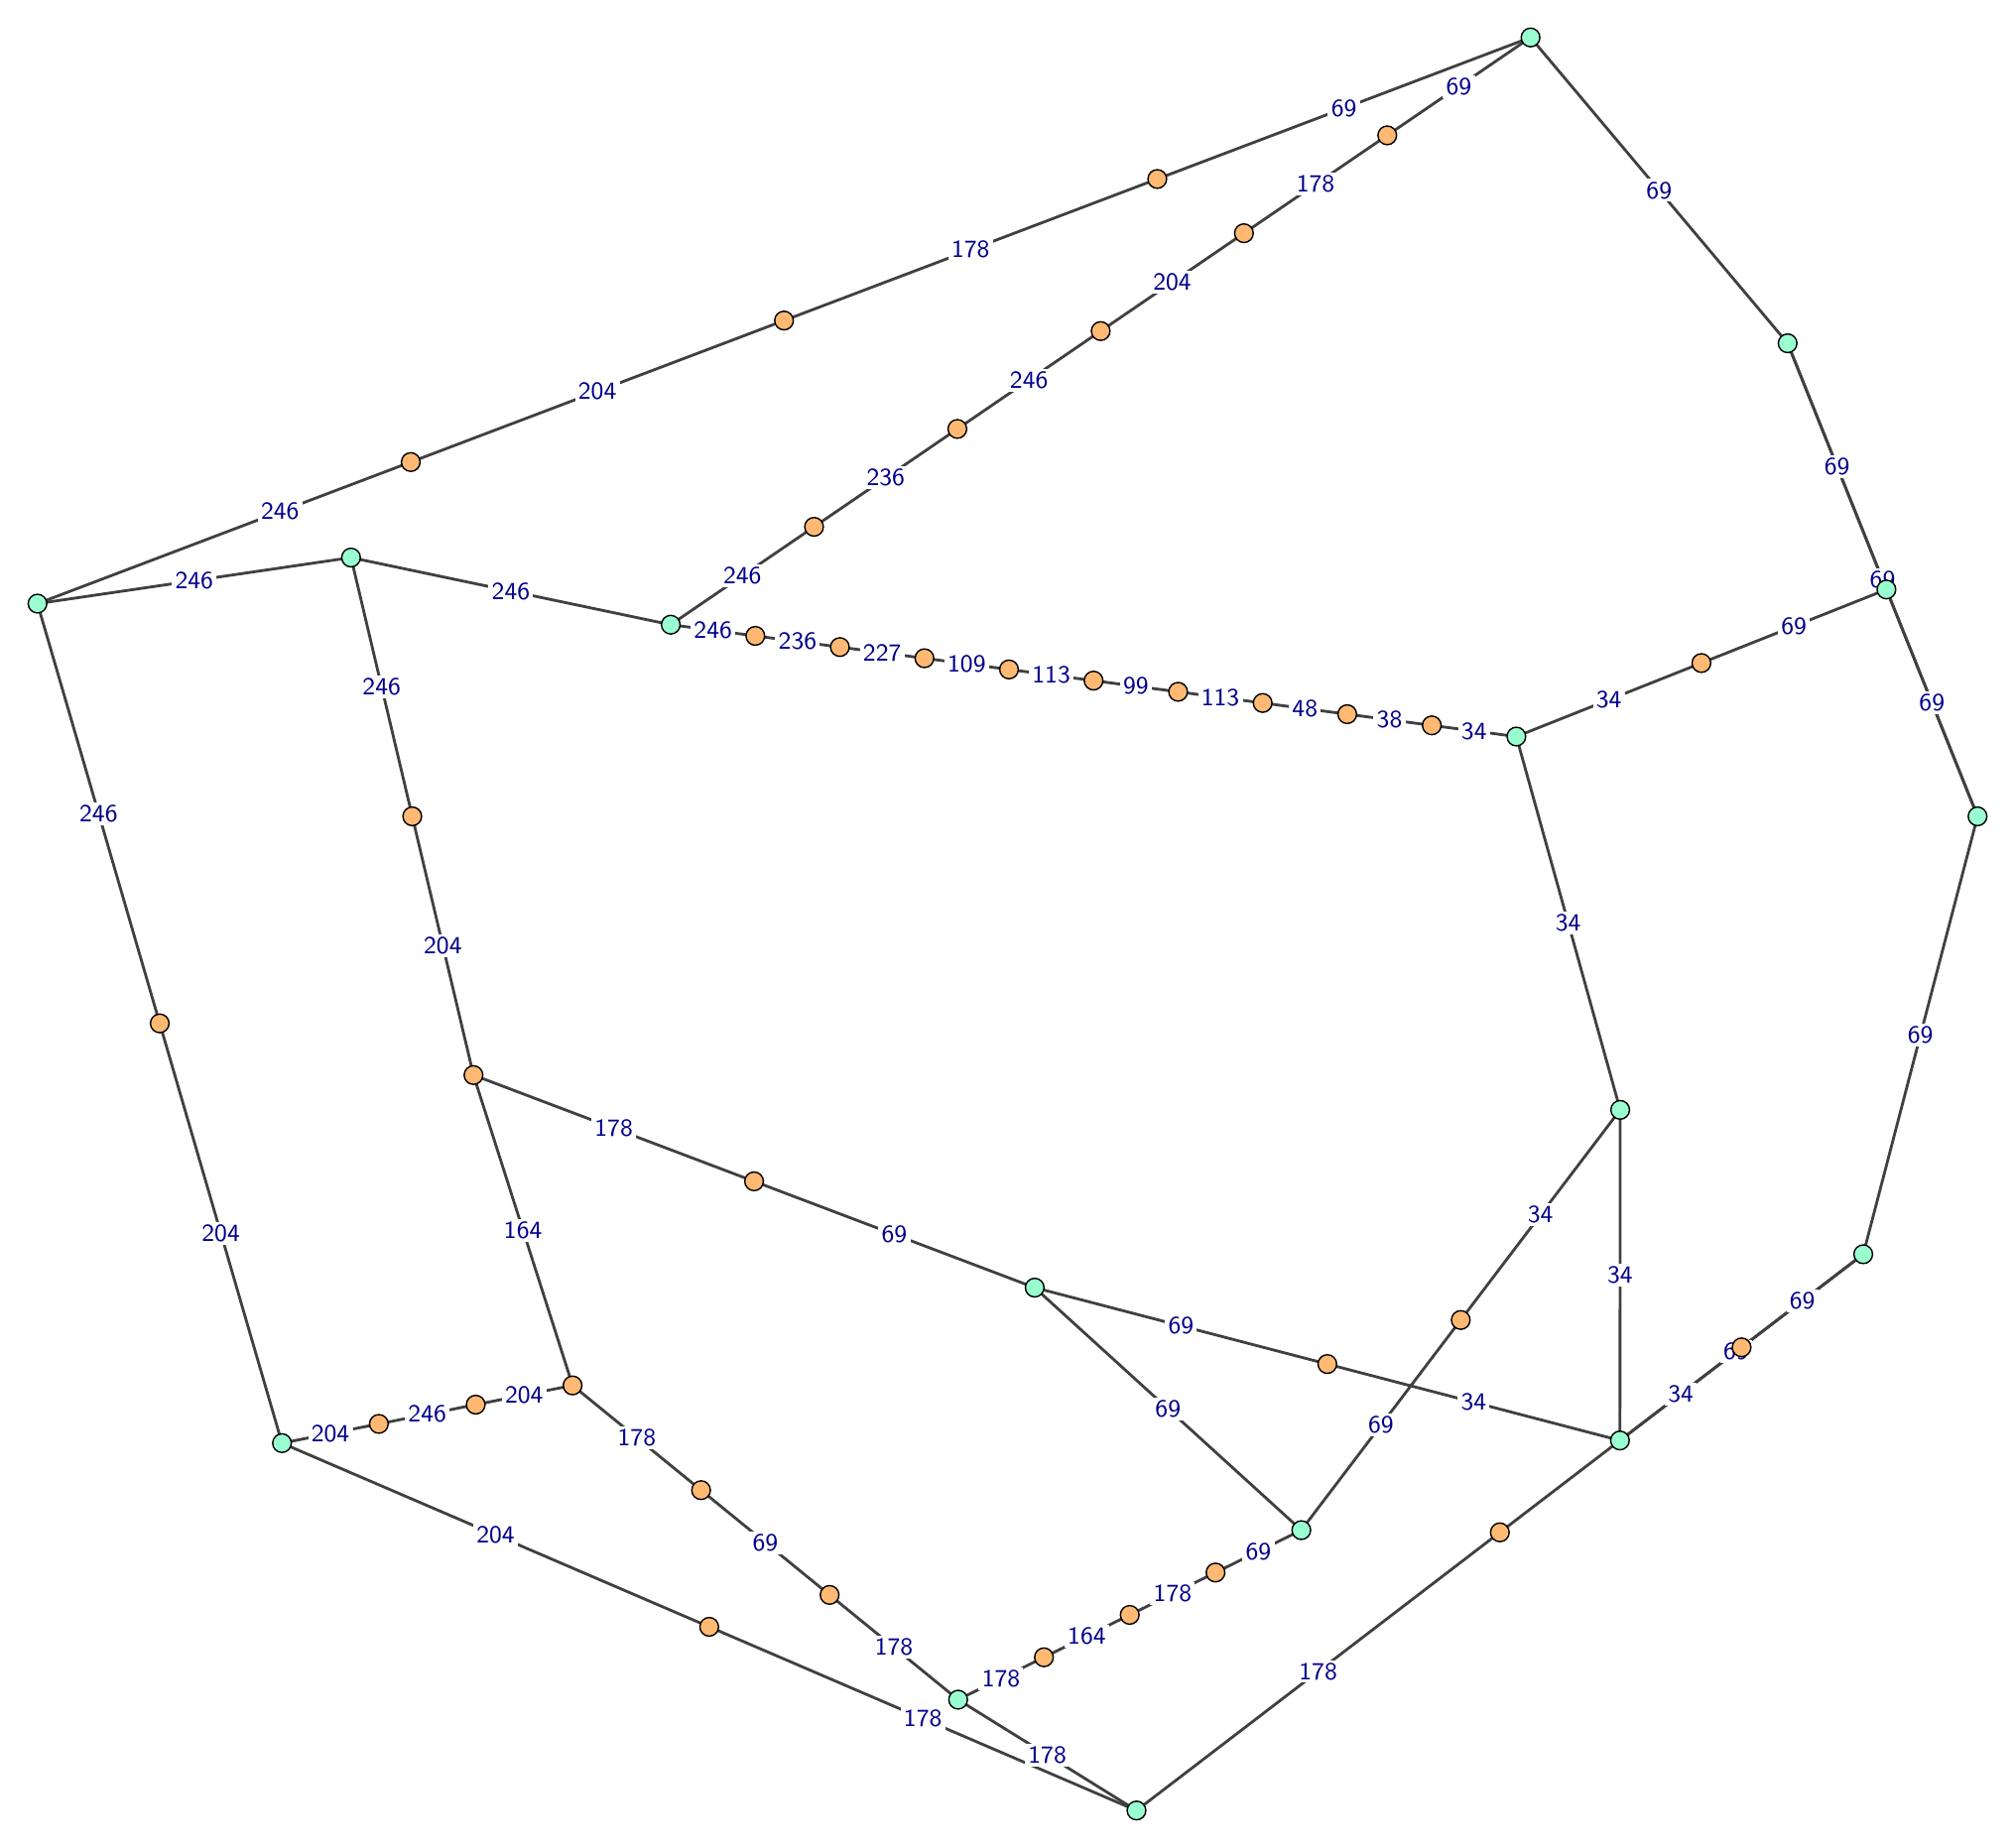
\begin{tikzpicture}[x=2.548738872546007cm,y=2.548738872546007cm]
\coordinate (c1) at (7.1481,2.4639);
\coordinate (c2) at (7.9489,3.5195);
\coordinate (c3) at (7.4274,5.3947);
\coordinate (c4) at (7.0027,5.4509);
\coordinate (c5) at (7.9477,1.8588);
\coordinate (c6) at (6.4780,2.2427);
\coordinate (c7) at (8.3567,5.7640);
\coordinate (c8) at (8.5586,2.3265);
\coordinate (c9) at (6.5780,5.5071);
\coordinate (c10) at (6.1533,5.5633);
\coordinate (c11) at (6.3474,1.4083);
\coordinate (c12) at (5.9165,1.1954);
\coordinate (c13) at (5.0083,2.6265);
\coordinate (c14) at (3.5990,3.1604);
\coordinate (c15) at (9.2860,6.1334);
\coordinate (c16) at (9.7436,4.9939);
\coordinate (c17) at (9.1696,2.7943);
\coordinate (c18) at (8.7899,7.3702);
\coordinate (c19) at (7.3446,1.3971);
\coordinate (c20) at (7.4987,8.9064);
\coordinate (c21) at (6.7790,8.4147);
\coordinate (c22) at (5.6240,8.1954);
\coordinate (c23) at (3.9783,1.0829);
\coordinate (c24) at (3.3328,1.6091);
\coordinate (c25) at (4.4546,5.7880);
\coordinate (c26) at (5.7286,5.6195);
\coordinate (c27) at (5.3039,5.6757);
\coordinate (c28) at (4.8793,5.7318);
\coordinate (c29) at (5.0547,0.7696);
\coordinate (c30) at (5.4856,0.9825);
\coordinate (c31) at (2.1897,3.6942);
\coordinate (c32) at (2.6874,2.1353);
\coordinate (c33) at (4.6238,0.5567);
\coordinate (c34) at (5.5196,0.0000);
\coordinate (c35) at (3.3738,0.9226);
\coordinate (c36) at (6.0593,7.9231);
\coordinate (c37) at (3.7493,7.4844);
\coordinate (c38) at (1.2280,1.8453);
\coordinate (c39) at (0.6140,3.9539);
\coordinate (c40) at (1.8822,4.9940);
\coordinate (c41) at (5.3396,7.4315);
\coordinate (c42) at (1.8747,6.7735);
\coordinate (c43) at (1.7145,1.9420);
\coordinate (c44) at (2.2009,2.0387);
\coordinate (c45) at (4.0299,5.8442);
\coordinate (c46) at (3.6052,5.9004);
\coordinate (c47) at (3.9002,6.4482);
\coordinate (c48) at (4.6199,6.9399);
\coordinate (c49) at (1.5747,6.2938);
\coordinate (c50) at (0.0000,6.0625);
\coordinate (c51) at (3.1805,5.9566);
\draw[curve edge] (c1) -- (c2);
\draw[curve edge] (c3) -- (c7);
\draw[curve edge] (c3) -- (c2);
\draw[curve edge] (c4) -- (c3);
\draw[curve edge] (c2) -- (c5);
\draw[curve edge] (c5) -- (c6);
\draw[curve edge] (c5) -- (c8);
\draw[curve edge] (c4) -- (c9);
\draw[curve edge] (c9) -- (c10);
\draw[curve edge] (c1) -- (c11);
\draw[curve edge] (c12) -- (c11);
\draw[curve edge] (c6) -- (c13);
\draw[curve edge] (c11) -- (c13);
\draw[curve edge] (c13) -- (c14);
\draw[curve edge] (c7) -- (c15);
\draw[curve edge] (c16) -- (c17);
\draw[curve edge] (c15) -- (c16);
\draw[curve edge] (c15) -- (c18);
\draw[curve edge] (c16) -- (c18);
\draw[curve edge] (c18) -- (c20);
\draw[curve edge] (c17) -- (c19);
\draw[curve edge] (c20) -- (c21);
\draw[curve edge] (c20) -- (c22);
\draw[curve edge] (c8) -- (c17);
\draw[curve edge] (c23) -- (c24);
\draw[curve edge] (c26) -- (c27);
\draw[curve edge] (c28) -- (c25);
\draw[curve edge] (c10) -- (c26);
\draw[curve edge] (c27) -- (c28);
\draw[curve edge] (c30) -- (c29);
\draw[curve edge] (c31) -- (c32);
\draw[curve edge] (c29) -- (c33);
\draw[curve edge] (c30) -- (c12);
\draw[curve edge] (c14) -- (c31);
\draw[curve edge] (c33) -- (c34);
\draw[curve edge] (c19) -- (c34);
\draw[curve edge] (c34) -- (c35);
\draw[curve edge] (c21) -- (c36);
\draw[curve edge] (c22) -- (c37);
\draw[curve edge] (c23) -- (c33);
\draw[curve edge] (c24) -- (c32);
\draw[curve edge] (c38) -- (c39);
\draw[curve edge] (c31) -- (c40);
\draw[curve edge] (c35) -- (c38);
\draw[curve edge] (c36) -- (c41);
\draw[curve edge] (c37) -- (c42);
\draw[curve edge] (c38) -- (c43);
\draw[curve edge] (c32) -- (c44);
\draw[curve edge] (c25) -- (c45);
\draw[curve edge] (c45) -- (c46);
\draw[curve edge] (c47) -- (c48);
\draw[curve edge] (c49) -- (c50);
\draw[curve edge] (c50) -- (c42);
\draw[curve edge] (c49) -- (c51);
\draw[curve edge] (c39) -- (c50);
\draw[curve edge] (c40) -- (c49);
\draw[curve edge] (c51) -- (c47);
\draw[curve edge] (c46) -- (c51);
\draw[curve edge] (c41) -- (c48);
\draw[curve edge] (c43) -- (c44);
\path (c1) -- node[curve cell,pos=0.5] {34} (c2);
\path (c3) -- node[curve cell,pos=0.5] {34} (c7);
\path (c3) -- node[curve cell,pos=0.5] {34} (c2);
\path (c4) -- node[curve cell,pos=0.5] {34} (c3);
\path (c2) -- node[curve cell,pos=0.5] {34} (c5);
\path (c5) -- node[curve cell,pos=0.5] {34} (c6);
\path (c5) -- node[curve cell,pos=0.5] {34} (c8);
\path (c4) -- node[curve cell,pos=0.5] {38} (c9);
\path (c9) -- node[curve cell,pos=0.5] {48} (c10);
\path (c1) -- node[curve cell,pos=0.5] {69} (c11);
\path (c12) -- node[curve cell,pos=0.5] {69} (c11);
\path (c6) -- node[curve cell,pos=0.5] {69} (c13);
\path (c11) -- node[curve cell,pos=0.5] {69} (c13);
\path (c13) -- node[curve cell,pos=0.5] {69} (c14);
\path (c7) -- node[curve cell,pos=0.5] {69} (c15);
\path (c16) -- node[curve cell,pos=0.5] {69} (c17);
\path (c15) -- node[curve cell,pos=0.5] {69} (c16);
\path (c15) -- node[curve cell,pos=0.5] {69} (c18);
\path (c16) -- node[curve cell,pos=0.5] {69} (c18);
\path (c18) -- node[curve cell,pos=0.5] {69} (c20);
\path (c17) -- node[curve cell,pos=0.35] {69} (c19);
\path (c20) -- node[curve cell,pos=0.5] {69} (c21);
\path (c20) -- node[curve cell,pos=0.5] {69} (c22);
\path (c8) -- node[curve cell,pos=0.5] {69} (c17);
\path (c23) -- node[curve cell,pos=0.5] {69} (c24);
\path (c26) -- node[curve cell,pos=0.5] {99} (c27);
\path (c28) -- node[curve cell,pos=0.5] {109} (c25);
\path (c10) -- node[curve cell,pos=0.5] {113} (c26);
\path (c27) -- node[curve cell,pos=0.5] {113} (c28);
\path (c30) -- node[curve cell,pos=0.5] {164} (c29);
\path (c31) -- node[curve cell,pos=0.5] {164} (c32);
\path (c29) -- node[curve cell,pos=0.5] {178} (c33);
\path (c30) -- node[curve cell,pos=0.5] {178} (c12);
\path (c14) -- node[curve cell,pos=0.5] {178} (c31);
\path (c33) -- node[curve cell,pos=0.5] {178} (c34);
\path (c19) -- node[curve cell,pos=0.5] {178} (c34);
\path (c34) -- node[curve cell,pos=0.5] {178} (c35);
\path (c21) -- node[curve cell,pos=0.5] {178} (c36);
\path (c22) -- node[curve cell,pos=0.5] {178} (c37);
\path (c23) -- node[curve cell,pos=0.5] {178} (c33);
\path (c24) -- node[curve cell,pos=0.5] {178} (c32);
\path (c38) -- node[curve cell,pos=0.5] {204} (c39);
\path (c31) -- node[curve cell,pos=0.5] {204} (c40);
\path (c35) -- node[curve cell,pos=0.5] {204} (c38);
\path (c36) -- node[curve cell,pos=0.5] {204} (c41);
\path (c37) -- node[curve cell,pos=0.5] {204} (c42);
\path (c38) -- node[curve cell,pos=0.5] {204} (c43);
\path (c32) -- node[curve cell,pos=0.5] {204} (c44);
\path (c25) -- node[curve cell,pos=0.5] {227} (c45);
\path (c45) -- node[curve cell,pos=0.5] {236} (c46);
\path (c47) -- node[curve cell,pos=0.5] {236} (c48);
\path (c49) -- node[curve cell,pos=0.5] {246} (c50);
\path (c50) -- node[curve cell,pos=0.65] {246} (c42);
\path (c49) -- node[curve cell,pos=0.5] {246} (c51);
\path (c39) -- node[curve cell,pos=0.5] {246} (c50);
\path (c40) -- node[curve cell,pos=0.5] {246} (c49);
\path (c51) -- node[curve cell,pos=0.5] {246} (c47);
\path (c46) -- node[curve cell,pos=0.5] {246} (c51);
\path (c41) -- node[curve cell,pos=0.5] {246} (c48);
\path (c43) -- node[curve cell,pos=0.5] {246} (c44);
\node[curve dot,curve g2 wall] at (c1) {};
\node[curve dot,curve bergman] at (c2) {};
\node[curve dot,curve bergman] at (c3) {};
\node[curve dot,curve g2 wall] at (c4) {};
\node[curve dot,curve bergman] at (c5) {};
\node[curve dot,curve g2 wall] at (c6) {};
\node[curve dot,curve g2 wall] at (c7) {};
\node[curve dot,curve g2 wall] at (c8) {};
\node[curve dot,curve g2 wall] at (c9) {};
\node[curve dot,curve g2 wall] at (c10) {};
\node[curve dot,curve bergman] at (c11) {};
\node[curve dot,curve g2 wall] at (c12) {};
\node[curve dot,curve bergman] at (c13) {};
\node[curve dot,curve g2 wall] at (c14) {};
\node[curve dot,curve bergman] at (c15) {};
\node[curve dot,curve bergman] at (c16) {};
\node[curve dot,curve bergman] at (c17) {};
\node[curve dot,curve bergman] at (c18) {};
\node[curve dot,curve g2 wall] at (c19) {};
\node[curve dot,curve bergman] at (c20) {};
\node[curve dot,curve g2 wall] at (c21) {};
\node[curve dot,curve g2 wall] at (c22) {};
\node[curve dot,curve g2 wall] at (c23) {};
\node[curve dot,curve g2 wall] at (c24) {};
\node[curve dot,curve g2 wall] at (c25) {};
\node[curve dot,curve g2 wall] at (c26) {};
\node[curve dot,curve g2 wall] at (c27) {};
\node[curve dot,curve g2 wall] at (c28) {};
\node[curve dot,curve g2 wall] at (c29) {};
\node[curve dot,curve g2 wall] at (c30) {};
\node[curve dot,curve g2 wall] at (c31) {};
\node[curve dot,curve g2 wall] at (c32) {};
\node[curve dot,curve bergman] at (c33) {};
\node[curve dot,curve bergman] at (c34) {};
\node[curve dot,curve g2 wall] at (c35) {};
\node[curve dot,curve g2 wall] at (c36) {};
\node[curve dot,curve g2 wall] at (c37) {};
\node[curve dot,curve bergman] at (c38) {};
\node[curve dot,curve g2 wall] at (c39) {};
\node[curve dot,curve g2 wall] at (c40) {};
\node[curve dot,curve g2 wall] at (c41) {};
\node[curve dot,curve g2 wall] at (c42) {};
\node[curve dot,curve g2 wall] at (c43) {};
\node[curve dot,curve g2 wall] at (c44) {};
\node[curve dot,curve g2 wall] at (c45) {};
\node[curve dot,curve g2 wall] at (c46) {};
\node[curve dot,curve g2 wall] at (c47) {};
\node[curve dot,curve g2 wall] at (c48) {};
\node[curve dot,curve bergman] at (c49) {};
\node[curve dot,curve bergman] at (c50) {};
\node[curve dot,curve bergman] at (c51) {};
\end{tikzpicture}
\vfill\clearpage
{\LARGE\bfseries The 13 maximal cells}\par\medskip
The G\(_2\)-tree of each cell, of the sum of the balanced generators of its rays, as in the tables of maximal
trees of \texttt{main.tex}; cells ordered by their number there. Below each tree, its edges and legs, counted.\par\bigskip
{\raggedright\setlength{\lineskip}{7mm}\lineskiplimit=0pt
\begin{minipage}[t]{6.2cm}\centering
{\large\bfseries cell 69}\\[1pt]{\small orbit 22, Type 7}\\[3pt]
\begingroup
\definecolor{g2TaxonBlue}{HTML}{1676A3}
\definecolor{g2TaxonYellow}{HTML}{E39A24}
\definecolor{g2HeartRed}{HTML}{D7443E}
\tikzset{
  g2tree pendant/.style={draw=black,line width=.6pt,line cap=round},
  g2tree internal/.style={draw=black,line width=2pt,line cap=round},
  g2tree vertex/.style={circle,fill=black,draw=white,line width=.4pt,inner sep=0pt,minimum size=3.8pt},
  g2tree dark/.style={fill=g2TaxonBlue,draw=white,line width=.55pt,text=white,inner sep=0pt},
  g2tree light/.style={fill=g2TaxonYellow,draw=white,line width=.55pt,text=white,inner sep=0pt},
  g2tree weight/.style={circle,fill=white,draw=none,text=black,inner sep=.15pt,minimum size=8.5pt},
  g2tree aligned pendant/.style={fill=white,text=black,inner sep=.7pt,sloped,above=1pt,font={\sffamily\fontsize{7.5}{8}\selectfont}},
  g2tree aligned internal/.style={fill=white,text=black,inner sep=1pt,sloped,above=1pt,font={\sffamily\fontsize{7.5}{8}\selectfont\bfseries}},
}
\begin{tikzpicture}[x=1.0cm,y=1.0cm,baseline=(current bounding box.center)]
\coordinate (v1) at (1.65748,1.32180);
\coordinate (v2) at (2.06685,-0.47174);
\coordinate (v3) at (0.91983,-1.91005);
\coordinate (v4) at (-1.65748,1.32180);
\coordinate (v5) at (-0.91983,-1.91005);
\coordinate (v6) at (-2.06685,-0.47174);
\coordinate (v7) at (0.00000,2.12000);
\coordinate (v8) at (0.81125,-0.46786);
\coordinate (v9) at (0.62523,0.20697);
\coordinate (v10) at (-0.00000,0.52176);
\coordinate (v11) at (-0.62523,0.20697);
\coordinate (v12) at (-0.81125,-0.46786);
\draw[g2tree internal] (v8)--(v9);
\draw[g2tree internal] (v9)--(v10);
\draw[g2tree internal] (v10)--(v11);
\draw[g2tree internal] (v11)--(v12);
\draw[g2tree pendant] (v1)--(v9);
\draw[g2tree pendant] (v2)--(v8);
\draw[g2tree pendant] (v3)--(v8);
\draw[g2tree pendant] (v4)--(v11);
\draw[g2tree pendant] (v5)--(v12);
\draw[g2tree pendant] (v6)--(v12);
\draw[g2tree pendant] (v7)--(v10);
\node[g2tree weight,font={\sffamily\fontsize{7.5}{8}\selectfont}] at (0.71824,-0.13044) {1};
\node[g2tree weight,font={\sffamily\fontsize{7.5}{8}\selectfont}] at (0.31261,0.36437) {3};
\node[g2tree weight,font={\sffamily\fontsize{7.5}{8}\selectfont}] at (-0.31261,0.36437) {3};
\node[g2tree weight,font={\sffamily\fontsize{7.5}{8}\selectfont}] at (-0.71824,-0.13044) {1};
\node[g2tree weight,font={\sffamily\fontsize{7.5}{8}\selectfont}] at (1.14135,0.76439) {3};
\node[g2tree weight,font={\sffamily\fontsize{7.5}{8}\selectfont}] at (1.43905,-0.46980) {3};
\node[g2tree weight,font={\sffamily\fontsize{7.5}{8}\selectfont}] at (0.86554,-1.18895) {3};
\node[g2tree weight,font={\sffamily\fontsize{7.5}{8}\selectfont}] at (-1.14135,0.76439) {3};
\node[g2tree weight,font={\sffamily\fontsize{7.5}{8}\selectfont}] at (-0.86554,-1.18895) {3};
\node[g2tree weight,font={\sffamily\fontsize{7.5}{8}\selectfont}] at (-1.43905,-0.46980) {3};
\node[g2tree weight,font={\sffamily\fontsize{7.5}{8}\selectfont}] at (0.00000,1.32088) {0};
\node[g2tree vertex] at (v8) {};
\node[g2tree vertex] at (v9) {};
\node[g2tree vertex] at (v10) {};
\node[g2tree vertex] at (v11) {};
\node[g2tree vertex] at (v12) {};
\node[g2tree dark,rectangle,minimum size=4.968mm,font={\sffamily\fontsize{9.6}{9.6}\selectfont\bfseries}] at (v1) {1};
\begin{scope}[shift={(v2)},scale=1.08,transform shape]
\path[fill=g2TaxonBlue,draw=white,line width=.55pt,line join=round] (0mm,3.0mm)--(-3.0mm,-2.2mm)--(3.0mm,-2.2mm)--cycle;
\node[font={\sffamily\fontsize{8.888888888888888}{8.888888888888888}\selectfont\bfseries},text=white,inner sep=0pt] at (0mm,-.35mm) {2};
\end{scope}
\node[g2tree dark,circle,minimum size=5.184mm,font={\sffamily\fontsize{9.6}{9.6}\selectfont\bfseries}] at (v3) {3};
\node[g2tree light,rectangle,minimum size=4.968mm,font={\sffamily\fontsize{9.6}{9.6}\selectfont\bfseries}] at (v4) {4};
\begin{scope}[shift={(v5)},scale=1.08,transform shape]
\path[fill=g2TaxonYellow,draw=white,line width=.55pt,line join=round] (0mm,3.0mm)--(-3.0mm,-2.2mm)--(3.0mm,-2.2mm)--cycle;
\node[font={\sffamily\fontsize{8.888888888888888}{8.888888888888888}\selectfont\bfseries},text=white,inner sep=0pt] at (0mm,-.35mm) {5};
\end{scope}
\node[g2tree light,circle,minimum size=5.184mm,font={\sffamily\fontsize{9.6}{9.6}\selectfont\bfseries}] at (v6) {6};
\begin{scope}[shift={(v7)},scale=1.08,transform shape]
\path[fill=g2HeartRed,draw=white,line width=.55pt]
  (0mm,-2.7mm)..controls(-.45mm,-2.1mm)and(-3.0mm,.35mm)..(-3.0mm,1.45mm)
  ..controls(-3.0mm,3.2mm)and(-.9mm,3.4mm)..(0mm,1.75mm)
  ..controls(.9mm,3.4mm)and(3.0mm,3.2mm)..(3.0mm,1.45mm)
  ..controls(3.0mm,.35mm)and(.45mm,-2.1mm)..(0mm,-2.7mm)--cycle;
\node[font={\sffamily\fontsize{8.888888888888888}{8.888888888888888}\selectfont\bfseries},text=white,inner sep=0pt] at (0mm,.35mm) {7};
\end{scope}
\end{tikzpicture}
\endgroup
\\[3pt]\scriptsize 16 edges.
\end{minipage}\hspace{6mm plus 4mm}%
\begin{minipage}[t]{6.2cm}\centering
{\large\bfseries cell 34}\\[1pt]{\small orbit 19, Type 12}\\[3pt]
\begingroup
\definecolor{g2TaxonBlue}{HTML}{1676A3}
\definecolor{g2TaxonYellow}{HTML}{E39A24}
\definecolor{g2HeartRed}{HTML}{D7443E}
\tikzset{
  g2tree pendant/.style={draw=black,line width=.6pt,line cap=round},
  g2tree internal/.style={draw=black,line width=2pt,line cap=round},
  g2tree vertex/.style={circle,fill=black,draw=white,line width=.4pt,inner sep=0pt,minimum size=3.8pt},
  g2tree dark/.style={fill=g2TaxonBlue,draw=white,line width=.55pt,text=white,inner sep=0pt},
  g2tree light/.style={fill=g2TaxonYellow,draw=white,line width=.55pt,text=white,inner sep=0pt},
  g2tree weight/.style={circle,fill=white,draw=none,text=black,inner sep=.15pt,minimum size=8.5pt},
  g2tree aligned pendant/.style={fill=white,text=black,inner sep=.7pt,sloped,above=1pt,font={\sffamily\fontsize{7.5}{8}\selectfont}},
  g2tree aligned internal/.style={fill=white,text=black,inner sep=1pt,sloped,above=1pt,font={\sffamily\fontsize{7.5}{8}\selectfont\bfseries}},
}
\begin{tikzpicture}[x=1.0cm,y=1.0cm,baseline=(current bounding box.center)]
\coordinate (v1) at (2.06685,-0.47174);
\coordinate (v2) at (0.91983,-1.91005);
\coordinate (v3) at (-0.91983,-1.91005);
\coordinate (v4) at (1.65748,1.32180);
\coordinate (v5) at (-2.06685,-0.47174);
\coordinate (v6) at (-1.65748,1.32180);
\coordinate (v7) at (0.00000,2.12000);
\coordinate (v8) at (0.14002,-0.92597);
\coordinate (v9) at (0.55164,-0.35978);
\coordinate (v10) at (0.40793,0.32531);
\coordinate (v11) at (-0.87159,0.34256);
\coordinate (v12) at (-0.22800,0.61787);
\draw[g2tree internal] (v8)--(v9);
\draw[g2tree internal] (v9)--(v10);
\draw[g2tree internal] (v10)--(v12);
\draw[g2tree internal] (v11)--(v12);
\draw[g2tree pendant] (v1)--(v9);
\draw[g2tree pendant] (v2)--(v8);
\draw[g2tree pendant] (v3)--(v8);
\draw[g2tree pendant] (v4)--(v10);
\draw[g2tree pendant] (v5)--(v11);
\draw[g2tree pendant] (v6)--(v11);
\draw[g2tree pendant] (v7)--(v12);
\node[g2tree weight,font={\sffamily\fontsize{7.5}{8}\selectfont}] at (0.34583,-0.64287) {1};
\node[g2tree weight,font={\sffamily\fontsize{7.5}{8}\selectfont}] at (0.47979,-0.01723) {3};
\node[g2tree weight,font={\sffamily\fontsize{7.5}{8}\selectfont}] at (0.08996,0.47159) {2};
\node[g2tree weight,font={\sffamily\fontsize{7.5}{8}\selectfont}] at (-0.54980,0.48021) {1};
\node[g2tree weight,font={\sffamily\fontsize{7.5}{8}\selectfont}] at (1.30924,-0.41576) {1};
\node[g2tree weight,font={\sffamily\fontsize{7.5}{8}\selectfont}] at (0.52993,-1.41801) {2};
\node[g2tree weight,font={\sffamily\fontsize{7.5}{8}\selectfont}] at (-0.38990,-1.41801) {2};
\node[g2tree weight,font={\sffamily\fontsize{7.5}{8}\selectfont}] at (1.03271,0.82356) {2};
\node[g2tree weight,font={\sffamily\fontsize{7.5}{8}\selectfont}] at (-1.46922,-0.06459) {3};
\node[g2tree weight,font={\sffamily\fontsize{7.5}{8}\selectfont}] at (-1.26454,0.83218) {3};
\node[g2tree weight,font={\sffamily\fontsize{7.5}{8}\selectfont}] at (-0.11400,1.36893) {0};
\node[g2tree vertex] at (v8) {};
\node[g2tree vertex] at (v9) {};
\node[g2tree vertex] at (v10) {};
\node[g2tree vertex] at (v11) {};
\node[g2tree vertex] at (v12) {};
\node[g2tree dark,rectangle,minimum size=4.968mm,font={\sffamily\fontsize{9.6}{9.6}\selectfont\bfseries}] at (v1) {1};
\begin{scope}[shift={(v2)},scale=1.08,transform shape]
\path[fill=g2TaxonBlue,draw=white,line width=.55pt,line join=round] (0mm,3.0mm)--(-3.0mm,-2.2mm)--(3.0mm,-2.2mm)--cycle;
\node[font={\sffamily\fontsize{8.888888888888888}{8.888888888888888}\selectfont\bfseries},text=white,inner sep=0pt] at (0mm,-.35mm) {2};
\end{scope}
\node[g2tree dark,circle,minimum size=5.184mm,font={\sffamily\fontsize{9.6}{9.6}\selectfont\bfseries}] at (v3) {3};
\node[g2tree light,rectangle,minimum size=4.968mm,font={\sffamily\fontsize{9.6}{9.6}\selectfont\bfseries}] at (v4) {4};
\begin{scope}[shift={(v5)},scale=1.08,transform shape]
\path[fill=g2TaxonYellow,draw=white,line width=.55pt,line join=round] (0mm,3.0mm)--(-3.0mm,-2.2mm)--(3.0mm,-2.2mm)--cycle;
\node[font={\sffamily\fontsize{8.888888888888888}{8.888888888888888}\selectfont\bfseries},text=white,inner sep=0pt] at (0mm,-.35mm) {5};
\end{scope}
\node[g2tree light,circle,minimum size=5.184mm,font={\sffamily\fontsize{9.6}{9.6}\selectfont\bfseries}] at (v6) {6};
\begin{scope}[shift={(v7)},scale=1.08,transform shape]
\path[fill=g2HeartRed,draw=white,line width=.55pt]
  (0mm,-2.7mm)..controls(-.45mm,-2.1mm)and(-3.0mm,.35mm)..(-3.0mm,1.45mm)
  ..controls(-3.0mm,3.2mm)and(-.9mm,3.4mm)..(0mm,1.75mm)
  ..controls(.9mm,3.4mm)and(3.0mm,3.2mm)..(3.0mm,1.45mm)
  ..controls(3.0mm,.35mm)and(.45mm,-2.1mm)..(0mm,-2.7mm)--cycle;
\node[font={\sffamily\fontsize{8.888888888888888}{8.888888888888888}\selectfont\bfseries},text=white,inner sep=0pt] at (0mm,.35mm) {7};
\end{scope}
\end{tikzpicture}
\endgroup
\\[3pt]\scriptsize 7 edges.
\end{minipage}\hspace{6mm plus 4mm}%
\begin{minipage}[t]{6.2cm}\centering
{\large\bfseries cell 178}\\[1pt]{\small orbit 19, Type 12}\\[3pt]
\begingroup
\definecolor{g2TaxonBlue}{HTML}{1676A3}
\definecolor{g2TaxonYellow}{HTML}{E39A24}
\definecolor{g2HeartRed}{HTML}{D7443E}
\tikzset{
  g2tree pendant/.style={draw=black,line width=.6pt,line cap=round},
  g2tree internal/.style={draw=black,line width=2pt,line cap=round},
  g2tree vertex/.style={circle,fill=black,draw=white,line width=.4pt,inner sep=0pt,minimum size=3.8pt},
  g2tree dark/.style={fill=g2TaxonBlue,draw=white,line width=.55pt,text=white,inner sep=0pt},
  g2tree light/.style={fill=g2TaxonYellow,draw=white,line width=.55pt,text=white,inner sep=0pt},
  g2tree weight/.style={circle,fill=white,draw=none,text=black,inner sep=.15pt,minimum size=8.5pt},
  g2tree aligned pendant/.style={fill=white,text=black,inner sep=.7pt,sloped,above=1pt,font={\sffamily\fontsize{7.5}{8}\selectfont}},
  g2tree aligned internal/.style={fill=white,text=black,inner sep=1pt,sloped,above=1pt,font={\sffamily\fontsize{7.5}{8}\selectfont\bfseries}},
}
\begin{tikzpicture}[x=1.0cm,y=1.0cm,baseline=(current bounding box.center)]
\coordinate (v1) at (1.65748,1.32180);
\coordinate (v2) at (-2.06685,-0.47174);
\coordinate (v3) at (-1.65748,1.32180);
\coordinate (v4) at (2.06685,-0.47174);
\coordinate (v5) at (0.91983,-1.91005);
\coordinate (v6) at (-0.91983,-1.91005);
\coordinate (v7) at (0.00000,2.12000);
\coordinate (v8) at (0.14002,-0.92597);
\coordinate (v9) at (0.55164,-0.35978);
\coordinate (v10) at (0.40793,0.32531);
\coordinate (v11) at (-0.87159,0.34256);
\coordinate (v12) at (-0.22800,0.61787);
\draw[g2tree internal] (v8)--(v9);
\draw[g2tree internal] (v9)--(v10);
\draw[g2tree internal] (v10)--(v12);
\draw[g2tree internal] (v11)--(v12);
\draw[g2tree pendant] (v1)--(v10);
\draw[g2tree pendant] (v2)--(v11);
\draw[g2tree pendant] (v3)--(v11);
\draw[g2tree pendant] (v4)--(v9);
\draw[g2tree pendant] (v5)--(v8);
\draw[g2tree pendant] (v6)--(v8);
\draw[g2tree pendant] (v7)--(v12);
\node[g2tree weight,font={\sffamily\fontsize{7.5}{8}\selectfont}] at (0.34583,-0.64287) {1};
\node[g2tree weight,font={\sffamily\fontsize{7.5}{8}\selectfont}] at (0.47979,-0.01723) {3};
\node[g2tree weight,font={\sffamily\fontsize{7.5}{8}\selectfont}] at (0.08996,0.47159) {2};
\node[g2tree weight,font={\sffamily\fontsize{7.5}{8}\selectfont}] at (-0.54980,0.48021) {1};
\node[g2tree weight,font={\sffamily\fontsize{7.5}{8}\selectfont}] at (1.03271,0.82356) {2};
\node[g2tree weight,font={\sffamily\fontsize{7.5}{8}\selectfont}] at (-1.46922,-0.06459) {3};
\node[g2tree weight,font={\sffamily\fontsize{7.5}{8}\selectfont}] at (-1.26454,0.83218) {3};
\node[g2tree weight,font={\sffamily\fontsize{7.5}{8}\selectfont}] at (1.30924,-0.41576) {1};
\node[g2tree weight,font={\sffamily\fontsize{7.5}{8}\selectfont}] at (0.52993,-1.41801) {2};
\node[g2tree weight,font={\sffamily\fontsize{7.5}{8}\selectfont}] at (-0.38990,-1.41801) {2};
\node[g2tree weight,font={\sffamily\fontsize{7.5}{8}\selectfont}] at (-0.11400,1.36893) {0};
\node[g2tree vertex] at (v8) {};
\node[g2tree vertex] at (v9) {};
\node[g2tree vertex] at (v10) {};
\node[g2tree vertex] at (v11) {};
\node[g2tree vertex] at (v12) {};
\node[g2tree dark,rectangle,minimum size=4.968mm,font={\sffamily\fontsize{9.6}{9.6}\selectfont\bfseries}] at (v1) {1};
\begin{scope}[shift={(v2)},scale=1.08,transform shape]
\path[fill=g2TaxonBlue,draw=white,line width=.55pt,line join=round] (0mm,3.0mm)--(-3.0mm,-2.2mm)--(3.0mm,-2.2mm)--cycle;
\node[font={\sffamily\fontsize{8.888888888888888}{8.888888888888888}\selectfont\bfseries},text=white,inner sep=0pt] at (0mm,-.35mm) {2};
\end{scope}
\node[g2tree dark,circle,minimum size=5.184mm,font={\sffamily\fontsize{9.6}{9.6}\selectfont\bfseries}] at (v3) {3};
\node[g2tree light,rectangle,minimum size=4.968mm,font={\sffamily\fontsize{9.6}{9.6}\selectfont\bfseries}] at (v4) {4};
\begin{scope}[shift={(v5)},scale=1.08,transform shape]
\path[fill=g2TaxonYellow,draw=white,line width=.55pt,line join=round] (0mm,3.0mm)--(-3.0mm,-2.2mm)--(3.0mm,-2.2mm)--cycle;
\node[font={\sffamily\fontsize{8.888888888888888}{8.888888888888888}\selectfont\bfseries},text=white,inner sep=0pt] at (0mm,-.35mm) {5};
\end{scope}
\node[g2tree light,circle,minimum size=5.184mm,font={\sffamily\fontsize{9.6}{9.6}\selectfont\bfseries}] at (v6) {6};
\begin{scope}[shift={(v7)},scale=1.08,transform shape]
\path[fill=g2HeartRed,draw=white,line width=.55pt]
  (0mm,-2.7mm)..controls(-.45mm,-2.1mm)and(-3.0mm,.35mm)..(-3.0mm,1.45mm)
  ..controls(-3.0mm,3.2mm)and(-.9mm,3.4mm)..(0mm,1.75mm)
  ..controls(.9mm,3.4mm)and(3.0mm,3.2mm)..(3.0mm,1.45mm)
  ..controls(3.0mm,.35mm)and(.45mm,-2.1mm)..(0mm,-2.7mm)--cycle;
\node[font={\sffamily\fontsize{8.888888888888888}{8.888888888888888}\selectfont\bfseries},text=white,inner sep=0pt] at (0mm,.35mm) {7};
\end{scope}
\end{tikzpicture}
\endgroup
\\[3pt]\scriptsize 10 edges.
\end{minipage}\hspace{6mm plus 4mm}%
\begin{minipage}[t]{6.2cm}\centering
{\large\bfseries cell 48}\\[1pt]{\small orbit 1, Type 16}\\[3pt]
\begingroup
\definecolor{g2TaxonBlue}{HTML}{1676A3}
\definecolor{g2TaxonYellow}{HTML}{E39A24}
\definecolor{g2HeartRed}{HTML}{D7443E}
\tikzset{
  g2tree pendant/.style={draw=black,line width=.6pt,line cap=round},
  g2tree internal/.style={draw=black,line width=2pt,line cap=round},
  g2tree vertex/.style={circle,fill=black,draw=white,line width=.4pt,inner sep=0pt,minimum size=3.8pt},
  g2tree dark/.style={fill=g2TaxonBlue,draw=white,line width=.55pt,text=white,inner sep=0pt},
  g2tree light/.style={fill=g2TaxonYellow,draw=white,line width=.55pt,text=white,inner sep=0pt},
  g2tree weight/.style={circle,fill=white,draw=none,text=black,inner sep=.15pt,minimum size=8.5pt},
  g2tree aligned pendant/.style={fill=white,text=black,inner sep=.7pt,sloped,above=1pt,font={\sffamily\fontsize{7.5}{8}\selectfont}},
  g2tree aligned internal/.style={fill=white,text=black,inner sep=1pt,sloped,above=1pt,font={\sffamily\fontsize{7.5}{8}\selectfont\bfseries}},
}
\begin{tikzpicture}[x=1.0cm,y=1.0cm,baseline=(current bounding box.center)]
\coordinate (v1) at (1.65748,1.32180);
\coordinate (v2) at (-0.91983,-1.91005);
\coordinate (v3) at (2.06685,-0.47174);
\coordinate (v4) at (0.91983,-1.91005);
\coordinate (v5) at (-1.65748,1.32180);
\coordinate (v6) at (-2.06685,-0.47174);
\coordinate (v7) at (0.00000,2.12000);
\coordinate (v8) at (-0.52792,0.77351);
\coordinate (v9) at (0.93391,0.06953);
\coordinate (v10) at (0.47351,-0.45775);
\coordinate (v11) at (-0.22638,-0.47009);
\coordinate (v12) at (-0.65311,0.08480);
\draw[g2tree internal] (v8)--(v12);
\draw[g2tree internal] (v9)--(v10);
\draw[g2tree internal] (v10)--(v11);
\draw[g2tree internal] (v11)--(v12);
\draw[g2tree pendant] (v1)--(v9);
\draw[g2tree pendant] (v2)--(v11);
\draw[g2tree pendant] (v3)--(v9);
\draw[g2tree pendant] (v4)--(v10);
\draw[g2tree pendant] (v5)--(v8);
\draw[g2tree pendant] (v6)--(v12);
\draw[g2tree pendant] (v7)--(v8);
\node[g2tree weight,font={\sffamily\fontsize{7.5}{8}\selectfont}] at (-0.59051,0.42916) {5};
\node[g2tree weight,font={\sffamily\fontsize{7.5}{8}\selectfont}] at (0.70371,-0.19411) {3};
\node[g2tree weight,font={\sffamily\fontsize{7.5}{8}\selectfont}] at (0.12356,-0.46392) {2};
\node[g2tree weight,font={\sffamily\fontsize{7.5}{8}\selectfont}] at (-0.43975,-0.19265) {2};
\node[g2tree weight,font={\sffamily\fontsize{7.5}{8}\selectfont}] at (1.29570,0.69567) {1};
\node[g2tree weight,font={\sffamily\fontsize{7.5}{8}\selectfont}] at (-0.57311,-1.19007) {3};
\node[g2tree weight,font={\sffamily\fontsize{7.5}{8}\selectfont}] at (1.50038,-0.20111) {3};
\node[g2tree weight,font={\sffamily\fontsize{7.5}{8}\selectfont}] at (0.69667,-1.18390) {2};
\node[g2tree weight,font={\sffamily\fontsize{7.5}{8}\selectfont}] at (-1.09270,1.04766) {4};
\node[g2tree weight,font={\sffamily\fontsize{7.5}{8}\selectfont}] at (-1.35998,-0.19347) {4};
\node[g2tree weight,font={\sffamily\fontsize{7.5}{8}\selectfont}] at (-0.26396,1.44676) {0};
\node[g2tree vertex] at (v8) {};
\node[g2tree vertex] at (v9) {};
\node[g2tree vertex] at (v10) {};
\node[g2tree vertex] at (v11) {};
\node[g2tree vertex] at (v12) {};
\node[g2tree dark,rectangle,minimum size=4.968mm,font={\sffamily\fontsize{9.6}{9.6}\selectfont\bfseries}] at (v1) {1};
\begin{scope}[shift={(v2)},scale=1.08,transform shape]
\path[fill=g2TaxonBlue,draw=white,line width=.55pt,line join=round] (0mm,3.0mm)--(-3.0mm,-2.2mm)--(3.0mm,-2.2mm)--cycle;
\node[font={\sffamily\fontsize{8.888888888888888}{8.888888888888888}\selectfont\bfseries},text=white,inner sep=0pt] at (0mm,-.35mm) {2};
\end{scope}
\node[g2tree dark,circle,minimum size=5.184mm,font={\sffamily\fontsize{9.6}{9.6}\selectfont\bfseries}] at (v3) {3};
\node[g2tree light,rectangle,minimum size=4.968mm,font={\sffamily\fontsize{9.6}{9.6}\selectfont\bfseries}] at (v4) {4};
\begin{scope}[shift={(v5)},scale=1.08,transform shape]
\path[fill=g2TaxonYellow,draw=white,line width=.55pt,line join=round] (0mm,3.0mm)--(-3.0mm,-2.2mm)--(3.0mm,-2.2mm)--cycle;
\node[font={\sffamily\fontsize{8.888888888888888}{8.888888888888888}\selectfont\bfseries},text=white,inner sep=0pt] at (0mm,-.35mm) {5};
\end{scope}
\node[g2tree light,circle,minimum size=5.184mm,font={\sffamily\fontsize{9.6}{9.6}\selectfont\bfseries}] at (v6) {6};
\begin{scope}[shift={(v7)},scale=1.08,transform shape]
\path[fill=g2HeartRed,draw=white,line width=.55pt]
  (0mm,-2.7mm)..controls(-.45mm,-2.1mm)and(-3.0mm,.35mm)..(-3.0mm,1.45mm)
  ..controls(-3.0mm,3.2mm)and(-.9mm,3.4mm)..(0mm,1.75mm)
  ..controls(.9mm,3.4mm)and(3.0mm,3.2mm)..(3.0mm,1.45mm)
  ..controls(3.0mm,.35mm)and(.45mm,-2.1mm)..(0mm,-2.7mm)--cycle;
\node[font={\sffamily\fontsize{8.888888888888888}{8.888888888888888}\selectfont\bfseries},text=white,inner sep=0pt] at (0mm,.35mm) {7};
\end{scope}
\end{tikzpicture}
\endgroup
\\[3pt]\scriptsize 1 edge.
\end{minipage}\hspace{6mm plus 4mm}%
\begin{minipage}[t]{6.2cm}\centering
{\large\bfseries cell 246}\\[1pt]{\small orbit 1, Type 16}\\[3pt]
\begingroup
\definecolor{g2TaxonBlue}{HTML}{1676A3}
\definecolor{g2TaxonYellow}{HTML}{E39A24}
\definecolor{g2HeartRed}{HTML}{D7443E}
\tikzset{
  g2tree pendant/.style={draw=black,line width=.6pt,line cap=round},
  g2tree internal/.style={draw=black,line width=2pt,line cap=round},
  g2tree vertex/.style={circle,fill=black,draw=white,line width=.4pt,inner sep=0pt,minimum size=3.8pt},
  g2tree dark/.style={fill=g2TaxonBlue,draw=white,line width=.55pt,text=white,inner sep=0pt},
  g2tree light/.style={fill=g2TaxonYellow,draw=white,line width=.55pt,text=white,inner sep=0pt},
  g2tree weight/.style={circle,fill=white,draw=none,text=black,inner sep=.15pt,minimum size=8.5pt},
  g2tree aligned pendant/.style={fill=white,text=black,inner sep=.7pt,sloped,above=1pt,font={\sffamily\fontsize{7.5}{8}\selectfont}},
  g2tree aligned internal/.style={fill=white,text=black,inner sep=1pt,sloped,above=1pt,font={\sffamily\fontsize{7.5}{8}\selectfont\bfseries}},
}
\begin{tikzpicture}[x=1.0cm,y=1.0cm,baseline=(current bounding box.center)]
\coordinate (v1) at (-0.91983,-1.91005);
\coordinate (v2) at (1.65748,1.32180);
\coordinate (v3) at (2.06685,-0.47174);
\coordinate (v4) at (-1.65748,1.32180);
\coordinate (v5) at (0.91983,-1.91005);
\coordinate (v6) at (-2.06685,-0.47174);
\coordinate (v7) at (0.00000,2.12000);
\coordinate (v8) at (0.52792,0.77351);
\coordinate (v9) at (-0.93391,0.06953);
\coordinate (v10) at (-0.47351,-0.45775);
\coordinate (v11) at (0.65311,0.08480);
\coordinate (v12) at (0.22638,-0.47009);
\draw[g2tree internal] (v8)--(v11);
\draw[g2tree internal] (v9)--(v10);
\draw[g2tree internal] (v10)--(v12);
\draw[g2tree internal] (v11)--(v12);
\draw[g2tree pendant] (v1)--(v10);
\draw[g2tree pendant] (v2)--(v8);
\draw[g2tree pendant] (v3)--(v11);
\draw[g2tree pendant] (v4)--(v9);
\draw[g2tree pendant] (v5)--(v12);
\draw[g2tree pendant] (v6)--(v9);
\draw[g2tree pendant] (v7)--(v8);
\node[g2tree weight,font={\sffamily\fontsize{7.5}{8}\selectfont}] at (0.59051,0.42916) {5};
\node[g2tree weight,font={\sffamily\fontsize{7.5}{8}\selectfont}] at (-0.70371,-0.19411) {3};
\node[g2tree weight,font={\sffamily\fontsize{7.5}{8}\selectfont}] at (-0.12356,-0.46392) {2};
\node[g2tree weight,font={\sffamily\fontsize{7.5}{8}\selectfont}] at (0.43975,-0.19265) {2};
\node[g2tree weight,font={\sffamily\fontsize{7.5}{8}\selectfont}] at (-0.69667,-1.18390) {2};
\node[g2tree weight,font={\sffamily\fontsize{7.5}{8}\selectfont}] at (1.09270,1.04766) {4};
\node[g2tree weight,font={\sffamily\fontsize{7.5}{8}\selectfont}] at (1.35998,-0.19347) {4};
\node[g2tree weight,font={\sffamily\fontsize{7.5}{8}\selectfont}] at (-1.29570,0.69567) {1};
\node[g2tree weight,font={\sffamily\fontsize{7.5}{8}\selectfont}] at (0.57311,-1.19007) {3};
\node[g2tree weight,font={\sffamily\fontsize{7.5}{8}\selectfont}] at (-1.50038,-0.20111) {3};
\node[g2tree weight,font={\sffamily\fontsize{7.5}{8}\selectfont}] at (0.26396,1.44676) {0};
\node[g2tree vertex] at (v8) {};
\node[g2tree vertex] at (v9) {};
\node[g2tree vertex] at (v10) {};
\node[g2tree vertex] at (v11) {};
\node[g2tree vertex] at (v12) {};
\node[g2tree dark,rectangle,minimum size=4.968mm,font={\sffamily\fontsize{9.6}{9.6}\selectfont\bfseries}] at (v1) {1};
\begin{scope}[shift={(v2)},scale=1.08,transform shape]
\path[fill=g2TaxonBlue,draw=white,line width=.55pt,line join=round] (0mm,3.0mm)--(-3.0mm,-2.2mm)--(3.0mm,-2.2mm)--cycle;
\node[font={\sffamily\fontsize{8.888888888888888}{8.888888888888888}\selectfont\bfseries},text=white,inner sep=0pt] at (0mm,-.35mm) {2};
\end{scope}
\node[g2tree dark,circle,minimum size=5.184mm,font={\sffamily\fontsize{9.6}{9.6}\selectfont\bfseries}] at (v3) {3};
\node[g2tree light,rectangle,minimum size=4.968mm,font={\sffamily\fontsize{9.6}{9.6}\selectfont\bfseries}] at (v4) {4};
\begin{scope}[shift={(v5)},scale=1.08,transform shape]
\path[fill=g2TaxonYellow,draw=white,line width=.55pt,line join=round] (0mm,3.0mm)--(-3.0mm,-2.2mm)--(3.0mm,-2.2mm)--cycle;
\node[font={\sffamily\fontsize{8.888888888888888}{8.888888888888888}\selectfont\bfseries},text=white,inner sep=0pt] at (0mm,-.35mm) {5};
\end{scope}
\node[g2tree light,circle,minimum size=5.184mm,font={\sffamily\fontsize{9.6}{9.6}\selectfont\bfseries}] at (v6) {6};
\begin{scope}[shift={(v7)},scale=1.08,transform shape]
\path[fill=g2HeartRed,draw=white,line width=.55pt]
  (0mm,-2.7mm)..controls(-.45mm,-2.1mm)and(-3.0mm,.35mm)..(-3.0mm,1.45mm)
  ..controls(-3.0mm,3.2mm)and(-.9mm,3.4mm)..(0mm,1.75mm)
  ..controls(.9mm,3.4mm)and(3.0mm,3.2mm)..(3.0mm,1.45mm)
  ..controls(3.0mm,.35mm)and(.45mm,-2.1mm)..(0mm,-2.7mm)--cycle;
\node[font={\sffamily\fontsize{8.888888888888888}{8.888888888888888}\selectfont\bfseries},text=white,inner sep=0pt] at (0mm,.35mm) {7};
\end{scope}
\end{tikzpicture}
\endgroup
\\[3pt]\scriptsize 9 edges.
\end{minipage}\hspace{6mm plus 4mm}%
\begin{minipage}[t]{6.2cm}\centering
{\large\bfseries cell 38}\\[1pt]{\small orbit 8, Type 17}\\[3pt]
\begingroup
\definecolor{g2TaxonBlue}{HTML}{1676A3}
\definecolor{g2TaxonYellow}{HTML}{E39A24}
\definecolor{g2HeartRed}{HTML}{D7443E}
\tikzset{
  g2tree pendant/.style={draw=black,line width=.6pt,line cap=round},
  g2tree internal/.style={draw=black,line width=2pt,line cap=round},
  g2tree vertex/.style={circle,fill=black,draw=white,line width=.4pt,inner sep=0pt,minimum size=3.8pt},
  g2tree dark/.style={fill=g2TaxonBlue,draw=white,line width=.55pt,text=white,inner sep=0pt},
  g2tree light/.style={fill=g2TaxonYellow,draw=white,line width=.55pt,text=white,inner sep=0pt},
  g2tree weight/.style={circle,fill=white,draw=none,text=black,inner sep=.15pt,minimum size=8.5pt},
  g2tree aligned pendant/.style={fill=white,text=black,inner sep=.7pt,sloped,above=1pt,font={\sffamily\fontsize{7.5}{8}\selectfont}},
  g2tree aligned internal/.style={fill=white,text=black,inner sep=1pt,sloped,above=1pt,font={\sffamily\fontsize{7.5}{8}\selectfont\bfseries}},
}
\begin{tikzpicture}[x=1.0cm,y=1.0cm,baseline=(current bounding box.center)]
\coordinate (v1) at (0.91983,-1.91005);
\coordinate (v2) at (-0.91983,-1.91005);
\coordinate (v3) at (2.06685,-0.47174);
\coordinate (v4) at (-2.06685,-0.47174);
\coordinate (v5) at (1.65748,1.32180);
\coordinate (v6) at (-1.65748,1.32180);
\coordinate (v7) at (0.00000,2.12000);
\coordinate (v8) at (0.63665,-0.68681);
\coordinate (v9) at (-0.06266,-0.65561);
\coordinate (v10) at (0.27560,0.89502);
\coordinate (v11) at (-0.50868,-0.11610);
\coordinate (v12) at (-0.34091,0.56349);
\draw[g2tree internal] (v8)--(v9);
\draw[g2tree internal] (v9)--(v11);
\draw[g2tree internal] (v10)--(v12);
\draw[g2tree internal] (v11)--(v12);
\draw[g2tree pendant] (v1)--(v8);
\draw[g2tree pendant] (v2)--(v9);
\draw[g2tree pendant] (v3)--(v8);
\draw[g2tree pendant] (v4)--(v11);
\draw[g2tree pendant] (v5)--(v10);
\draw[g2tree pendant] (v6)--(v12);
\draw[g2tree pendant] (v7)--(v10);
\node[g2tree weight,font={\sffamily\fontsize{7.5}{8}\selectfont}] at (0.28699,-0.67121) {3};
\node[g2tree weight,font={\sffamily\fontsize{7.5}{8}\selectfont}] at (-0.28567,-0.38585) {3};
\node[g2tree weight,font={\sffamily\fontsize{7.5}{8}\selectfont}] at (-0.03265,0.72926) {3};
\node[g2tree weight,font={\sffamily\fontsize{7.5}{8}\selectfont}] at (-0.42480,0.22370) {2};
\node[g2tree weight,font={\sffamily\fontsize{7.5}{8}\selectfont}] at (0.77824,-1.29843) {2};
\node[g2tree weight,font={\sffamily\fontsize{7.5}{8}\selectfont}] at (-0.49125,-1.28283) {3};
\node[g2tree weight,font={\sffamily\fontsize{7.5}{8}\selectfont}] at (1.35175,-0.57927) {3};
\node[g2tree weight,font={\sffamily\fontsize{7.5}{8}\selectfont}] at (-1.28776,-0.29392) {4};
\node[g2tree weight,font={\sffamily\fontsize{7.5}{8}\selectfont}] at (0.96654,1.10841) {5};
\node[g2tree weight,font={\sffamily\fontsize{7.5}{8}\selectfont}] at (-0.99920,0.94265) {5};
\node[g2tree weight,font={\sffamily\fontsize{7.5}{8}\selectfont}] at (0.13780,1.50751) {0};
\node[g2tree vertex] at (v8) {};
\node[g2tree vertex] at (v9) {};
\node[g2tree vertex] at (v10) {};
\node[g2tree vertex] at (v11) {};
\node[g2tree vertex] at (v12) {};
\node[g2tree dark,rectangle,minimum size=4.968mm,font={\sffamily\fontsize{9.6}{9.6}\selectfont\bfseries}] at (v1) {1};
\begin{scope}[shift={(v2)},scale=1.08,transform shape]
\path[fill=g2TaxonBlue,draw=white,line width=.55pt,line join=round] (0mm,3.0mm)--(-3.0mm,-2.2mm)--(3.0mm,-2.2mm)--cycle;
\node[font={\sffamily\fontsize{8.888888888888888}{8.888888888888888}\selectfont\bfseries},text=white,inner sep=0pt] at (0mm,-.35mm) {2};
\end{scope}
\node[g2tree dark,circle,minimum size=5.184mm,font={\sffamily\fontsize{9.6}{9.6}\selectfont\bfseries}] at (v3) {3};
\node[g2tree light,rectangle,minimum size=4.968mm,font={\sffamily\fontsize{9.6}{9.6}\selectfont\bfseries}] at (v4) {4};
\begin{scope}[shift={(v5)},scale=1.08,transform shape]
\path[fill=g2TaxonYellow,draw=white,line width=.55pt,line join=round] (0mm,3.0mm)--(-3.0mm,-2.2mm)--(3.0mm,-2.2mm)--cycle;
\node[font={\sffamily\fontsize{8.888888888888888}{8.888888888888888}\selectfont\bfseries},text=white,inner sep=0pt] at (0mm,-.35mm) {5};
\end{scope}
\node[g2tree light,circle,minimum size=5.184mm,font={\sffamily\fontsize{9.6}{9.6}\selectfont\bfseries}] at (v6) {6};
\begin{scope}[shift={(v7)},scale=1.08,transform shape]
\path[fill=g2HeartRed,draw=white,line width=.55pt]
  (0mm,-2.7mm)..controls(-.45mm,-2.1mm)and(-3.0mm,.35mm)..(-3.0mm,1.45mm)
  ..controls(-3.0mm,3.2mm)and(-.9mm,3.4mm)..(0mm,1.75mm)
  ..controls(.9mm,3.4mm)and(3.0mm,3.2mm)..(3.0mm,1.45mm)
  ..controls(3.0mm,.35mm)and(.45mm,-2.1mm)..(0mm,-2.7mm)--cycle;
\node[font={\sffamily\fontsize{8.888888888888888}{8.888888888888888}\selectfont\bfseries},text=white,inner sep=0pt] at (0mm,.35mm) {7};
\end{scope}
\end{tikzpicture}
\endgroup
\\[3pt]\scriptsize 1 edge.
\end{minipage}\hspace{6mm plus 4mm}%
\begin{minipage}[t]{6.2cm}\centering
{\large\bfseries cell 164}\\[1pt]{\small orbit 8, Type 17}\\[3pt]
\begingroup
\definecolor{g2TaxonBlue}{HTML}{1676A3}
\definecolor{g2TaxonYellow}{HTML}{E39A24}
\definecolor{g2HeartRed}{HTML}{D7443E}
\tikzset{
  g2tree pendant/.style={draw=black,line width=.6pt,line cap=round},
  g2tree internal/.style={draw=black,line width=2pt,line cap=round},
  g2tree vertex/.style={circle,fill=black,draw=white,line width=.4pt,inner sep=0pt,minimum size=3.8pt},
  g2tree dark/.style={fill=g2TaxonBlue,draw=white,line width=.55pt,text=white,inner sep=0pt},
  g2tree light/.style={fill=g2TaxonYellow,draw=white,line width=.55pt,text=white,inner sep=0pt},
  g2tree weight/.style={circle,fill=white,draw=none,text=black,inner sep=.15pt,minimum size=8.5pt},
  g2tree aligned pendant/.style={fill=white,text=black,inner sep=.7pt,sloped,above=1pt,font={\sffamily\fontsize{7.5}{8}\selectfont}},
  g2tree aligned internal/.style={fill=white,text=black,inner sep=1pt,sloped,above=1pt,font={\sffamily\fontsize{7.5}{8}\selectfont\bfseries}},
}
\begin{tikzpicture}[x=1.0cm,y=1.0cm,baseline=(current bounding box.center)]
\coordinate (v1) at (2.06685,-0.47174);
\coordinate (v2) at (1.65748,1.32180);
\coordinate (v3) at (-1.65748,1.32180);
\coordinate (v4) at (-0.91983,-1.91005);
\coordinate (v5) at (-2.06685,-0.47174);
\coordinate (v6) at (0.91983,-1.91005);
\coordinate (v7) at (0.00000,2.12000);
\coordinate (v8) at (-0.63665,-0.68681);
\coordinate (v9) at (-0.27560,0.89502);
\coordinate (v10) at (0.06266,-0.65561);
\coordinate (v11) at (0.50868,-0.11610);
\coordinate (v12) at (0.34091,0.56349);
\draw[g2tree internal] (v8)--(v10);
\draw[g2tree internal] (v9)--(v12);
\draw[g2tree internal] (v10)--(v11);
\draw[g2tree internal] (v11)--(v12);
\draw[g2tree pendant] (v1)--(v11);
\draw[g2tree pendant] (v2)--(v12);
\draw[g2tree pendant] (v3)--(v9);
\draw[g2tree pendant] (v4)--(v8);
\draw[g2tree pendant] (v5)--(v8);
\draw[g2tree pendant] (v6)--(v10);
\draw[g2tree pendant] (v7)--(v9);
\node[g2tree weight,font={\sffamily\fontsize{7.5}{8}\selectfont}] at (-0.28699,-0.67121) {3};
\node[g2tree weight,font={\sffamily\fontsize{7.5}{8}\selectfont}] at (0.03265,0.72926) {3};
\node[g2tree weight,font={\sffamily\fontsize{7.5}{8}\selectfont}] at (0.28567,-0.38585) {3};
\node[g2tree weight,font={\sffamily\fontsize{7.5}{8}\selectfont}] at (0.42480,0.22370) {2};
\node[g2tree weight,font={\sffamily\fontsize{7.5}{8}\selectfont}] at (1.28776,-0.29392) {4};
\node[g2tree weight,font={\sffamily\fontsize{7.5}{8}\selectfont}] at (0.99920,0.94265) {5};
\node[g2tree weight,font={\sffamily\fontsize{7.5}{8}\selectfont}] at (-0.96654,1.10841) {5};
\node[g2tree weight,font={\sffamily\fontsize{7.5}{8}\selectfont}] at (-0.77824,-1.29843) {2};
\node[g2tree weight,font={\sffamily\fontsize{7.5}{8}\selectfont}] at (-1.35175,-0.57927) {3};
\node[g2tree weight,font={\sffamily\fontsize{7.5}{8}\selectfont}] at (0.49125,-1.28283) {3};
\node[g2tree weight,font={\sffamily\fontsize{7.5}{8}\selectfont}] at (-0.13780,1.50751) {0};
\node[g2tree vertex] at (v8) {};
\node[g2tree vertex] at (v9) {};
\node[g2tree vertex] at (v10) {};
\node[g2tree vertex] at (v11) {};
\node[g2tree vertex] at (v12) {};
\node[g2tree dark,rectangle,minimum size=4.968mm,font={\sffamily\fontsize{9.6}{9.6}\selectfont\bfseries}] at (v1) {1};
\begin{scope}[shift={(v2)},scale=1.08,transform shape]
\path[fill=g2TaxonBlue,draw=white,line width=.55pt,line join=round] (0mm,3.0mm)--(-3.0mm,-2.2mm)--(3.0mm,-2.2mm)--cycle;
\node[font={\sffamily\fontsize{8.888888888888888}{8.888888888888888}\selectfont\bfseries},text=white,inner sep=0pt] at (0mm,-.35mm) {2};
\end{scope}
\node[g2tree dark,circle,minimum size=5.184mm,font={\sffamily\fontsize{9.6}{9.6}\selectfont\bfseries}] at (v3) {3};
\node[g2tree light,rectangle,minimum size=4.968mm,font={\sffamily\fontsize{9.6}{9.6}\selectfont\bfseries}] at (v4) {4};
\begin{scope}[shift={(v5)},scale=1.08,transform shape]
\path[fill=g2TaxonYellow,draw=white,line width=.55pt,line join=round] (0mm,3.0mm)--(-3.0mm,-2.2mm)--(3.0mm,-2.2mm)--cycle;
\node[font={\sffamily\fontsize{8.888888888888888}{8.888888888888888}\selectfont\bfseries},text=white,inner sep=0pt] at (0mm,-.35mm) {5};
\end{scope}
\node[g2tree light,circle,minimum size=5.184mm,font={\sffamily\fontsize{9.6}{9.6}\selectfont\bfseries}] at (v6) {6};
\begin{scope}[shift={(v7)},scale=1.08,transform shape]
\path[fill=g2HeartRed,draw=white,line width=.55pt]
  (0mm,-2.7mm)..controls(-.45mm,-2.1mm)and(-3.0mm,.35mm)..(-3.0mm,1.45mm)
  ..controls(-3.0mm,3.2mm)and(-.9mm,3.4mm)..(0mm,1.75mm)
  ..controls(.9mm,3.4mm)and(3.0mm,3.2mm)..(3.0mm,1.45mm)
  ..controls(3.0mm,.35mm)and(.45mm,-2.1mm)..(0mm,-2.7mm)--cycle;
\node[font={\sffamily\fontsize{8.888888888888888}{8.888888888888888}\selectfont\bfseries},text=white,inner sep=0pt] at (0mm,.35mm) {7};
\end{scope}
\end{tikzpicture}
\endgroup
\\[3pt]\scriptsize 2 edges.
\end{minipage}\hspace{6mm plus 4mm}%
\begin{minipage}[t]{6.2cm}\centering
{\large\bfseries cell 204}\\[1pt]{\small orbit 8, Type 17}\\[3pt]
\begingroup
\definecolor{g2TaxonBlue}{HTML}{1676A3}
\definecolor{g2TaxonYellow}{HTML}{E39A24}
\definecolor{g2HeartRed}{HTML}{D7443E}
\tikzset{
  g2tree pendant/.style={draw=black,line width=.6pt,line cap=round},
  g2tree internal/.style={draw=black,line width=2pt,line cap=round},
  g2tree vertex/.style={circle,fill=black,draw=white,line width=.4pt,inner sep=0pt,minimum size=3.8pt},
  g2tree dark/.style={fill=g2TaxonBlue,draw=white,line width=.55pt,text=white,inner sep=0pt},
  g2tree light/.style={fill=g2TaxonYellow,draw=white,line width=.55pt,text=white,inner sep=0pt},
  g2tree weight/.style={circle,fill=white,draw=none,text=black,inner sep=.15pt,minimum size=8.5pt},
  g2tree aligned pendant/.style={fill=white,text=black,inner sep=.7pt,sloped,above=1pt,font={\sffamily\fontsize{7.5}{8}\selectfont}},
  g2tree aligned internal/.style={fill=white,text=black,inner sep=1pt,sloped,above=1pt,font={\sffamily\fontsize{7.5}{8}\selectfont\bfseries}},
}
\begin{tikzpicture}[x=1.0cm,y=1.0cm,baseline=(current bounding box.center)]
\coordinate (v1) at (-2.06685,-0.47174);
\coordinate (v2) at (1.65748,1.32180);
\coordinate (v3) at (-1.65748,1.32180);
\coordinate (v4) at (0.91983,-1.91005);
\coordinate (v5) at (-0.91983,-1.91005);
\coordinate (v6) at (2.06685,-0.47174);
\coordinate (v7) at (0.00000,2.12000);
\coordinate (v8) at (0.63665,-0.68681);
\coordinate (v9) at (0.27560,0.89502);
\coordinate (v10) at (-0.06266,-0.65561);
\coordinate (v11) at (-0.50868,-0.11610);
\coordinate (v12) at (-0.34091,0.56349);
\draw[g2tree internal] (v8)--(v10);
\draw[g2tree internal] (v9)--(v12);
\draw[g2tree internal] (v10)--(v11);
\draw[g2tree internal] (v11)--(v12);
\draw[g2tree pendant] (v1)--(v11);
\draw[g2tree pendant] (v2)--(v9);
\draw[g2tree pendant] (v3)--(v12);
\draw[g2tree pendant] (v4)--(v8);
\draw[g2tree pendant] (v5)--(v10);
\draw[g2tree pendant] (v6)--(v8);
\draw[g2tree pendant] (v7)--(v9);
\node[g2tree weight,font={\sffamily\fontsize{7.5}{8}\selectfont}] at (0.28699,-0.67121) {3};
\node[g2tree weight,font={\sffamily\fontsize{7.5}{8}\selectfont}] at (-0.03265,0.72926) {3};
\node[g2tree weight,font={\sffamily\fontsize{7.5}{8}\selectfont}] at (-0.28567,-0.38585) {3};
\node[g2tree weight,font={\sffamily\fontsize{7.5}{8}\selectfont}] at (-0.42480,0.22370) {2};
\node[g2tree weight,font={\sffamily\fontsize{7.5}{8}\selectfont}] at (-1.28776,-0.29392) {4};
\node[g2tree weight,font={\sffamily\fontsize{7.5}{8}\selectfont}] at (0.96654,1.10841) {5};
\node[g2tree weight,font={\sffamily\fontsize{7.5}{8}\selectfont}] at (-0.99920,0.94265) {5};
\node[g2tree weight,font={\sffamily\fontsize{7.5}{8}\selectfont}] at (0.77824,-1.29843) {2};
\node[g2tree weight,font={\sffamily\fontsize{7.5}{8}\selectfont}] at (-0.49125,-1.28283) {3};
\node[g2tree weight,font={\sffamily\fontsize{7.5}{8}\selectfont}] at (1.35175,-0.57927) {3};
\node[g2tree weight,font={\sffamily\fontsize{7.5}{8}\selectfont}] at (0.13780,1.50751) {0};
\node[g2tree vertex] at (v8) {};
\node[g2tree vertex] at (v9) {};
\node[g2tree vertex] at (v10) {};
\node[g2tree vertex] at (v11) {};
\node[g2tree vertex] at (v12) {};
\node[g2tree dark,rectangle,minimum size=4.968mm,font={\sffamily\fontsize{9.6}{9.6}\selectfont\bfseries}] at (v1) {1};
\begin{scope}[shift={(v2)},scale=1.08,transform shape]
\path[fill=g2TaxonBlue,draw=white,line width=.55pt,line join=round] (0mm,3.0mm)--(-3.0mm,-2.2mm)--(3.0mm,-2.2mm)--cycle;
\node[font={\sffamily\fontsize{8.888888888888888}{8.888888888888888}\selectfont\bfseries},text=white,inner sep=0pt] at (0mm,-.35mm) {2};
\end{scope}
\node[g2tree dark,circle,minimum size=5.184mm,font={\sffamily\fontsize{9.6}{9.6}\selectfont\bfseries}] at (v3) {3};
\node[g2tree light,rectangle,minimum size=4.968mm,font={\sffamily\fontsize{9.6}{9.6}\selectfont\bfseries}] at (v4) {4};
\begin{scope}[shift={(v5)},scale=1.08,transform shape]
\path[fill=g2TaxonYellow,draw=white,line width=.55pt,line join=round] (0mm,3.0mm)--(-3.0mm,-2.2mm)--(3.0mm,-2.2mm)--cycle;
\node[font={\sffamily\fontsize{8.888888888888888}{8.888888888888888}\selectfont\bfseries},text=white,inner sep=0pt] at (0mm,-.35mm) {5};
\end{scope}
\node[g2tree light,circle,minimum size=5.184mm,font={\sffamily\fontsize{9.6}{9.6}\selectfont\bfseries}] at (v6) {6};
\begin{scope}[shift={(v7)},scale=1.08,transform shape]
\path[fill=g2HeartRed,draw=white,line width=.55pt]
  (0mm,-2.7mm)..controls(-.45mm,-2.1mm)and(-3.0mm,.35mm)..(-3.0mm,1.45mm)
  ..controls(-3.0mm,3.2mm)and(-.9mm,3.4mm)..(0mm,1.75mm)
  ..controls(.9mm,3.4mm)and(3.0mm,3.2mm)..(3.0mm,1.45mm)
  ..controls(3.0mm,.35mm)and(.45mm,-2.1mm)..(0mm,-2.7mm)--cycle;
\node[font={\sffamily\fontsize{8.888888888888888}{8.888888888888888}\selectfont\bfseries},text=white,inner sep=0pt] at (0mm,.35mm) {7};
\end{scope}
\end{tikzpicture}
\endgroup
\\[3pt]\scriptsize 7 edges.
\end{minipage}\hspace{6mm plus 4mm}%
\begin{minipage}[t]{6.2cm}\centering
{\large\bfseries cell 113}\\[1pt]{\small orbit 3, Type 22}\\[3pt]
\begingroup
\definecolor{g2TaxonBlue}{HTML}{1676A3}
\definecolor{g2TaxonYellow}{HTML}{E39A24}
\definecolor{g2HeartRed}{HTML}{D7443E}
\tikzset{
  g2tree pendant/.style={draw=black,line width=.6pt,line cap=round},
  g2tree internal/.style={draw=black,line width=2pt,line cap=round},
  g2tree vertex/.style={circle,fill=black,draw=white,line width=.4pt,inner sep=0pt,minimum size=3.8pt},
  g2tree dark/.style={fill=g2TaxonBlue,draw=white,line width=.55pt,text=white,inner sep=0pt},
  g2tree light/.style={fill=g2TaxonYellow,draw=white,line width=.55pt,text=white,inner sep=0pt},
  g2tree weight/.style={circle,fill=white,draw=none,text=black,inner sep=.15pt,minimum size=8.5pt},
  g2tree aligned pendant/.style={fill=white,text=black,inner sep=.7pt,sloped,above=1pt,font={\sffamily\fontsize{7.5}{8}\selectfont}},
  g2tree aligned internal/.style={fill=white,text=black,inner sep=1pt,sloped,above=1pt,font={\sffamily\fontsize{7.5}{8}\selectfont\bfseries}},
}
\begin{tikzpicture}[x=1.0cm,y=1.0cm,baseline=(current bounding box.center)]
\coordinate (v1) at (1.65748,1.32180);
\coordinate (v2) at (-2.06685,-0.47174);
\coordinate (v3) at (2.06685,-0.47174);
\coordinate (v4) at (0.91983,-1.91005);
\coordinate (v5) at (-1.65748,1.32180);
\coordinate (v6) at (-0.91983,-1.91005);
\coordinate (v7) at (0.00000,2.12000);
\coordinate (v8) at (-0.52792,0.77351);
\coordinate (v9) at (0.93391,0.06953);
\coordinate (v10) at (0.47351,-0.45775);
\coordinate (v11) at (-0.65311,0.08480);
\coordinate (v12) at (-0.22638,-0.47009);
\draw[g2tree internal] (v8)--(v11);
\draw[g2tree internal] (v9)--(v10);
\draw[g2tree internal] (v10)--(v12);
\draw[g2tree internal] (v11)--(v12);
\draw[g2tree pendant] (v1)--(v9);
\draw[g2tree pendant] (v2)--(v11);
\draw[g2tree pendant] (v3)--(v9);
\draw[g2tree pendant] (v4)--(v10);
\draw[g2tree pendant] (v5)--(v8);
\draw[g2tree pendant] (v6)--(v12);
\draw[g2tree pendant] (v7)--(v8);
\node[g2tree weight,font={\sffamily\fontsize{7.5}{8}\selectfont}] at (-0.59051,0.42916) {5};
\node[g2tree weight,font={\sffamily\fontsize{7.5}{8}\selectfont}] at (0.70371,-0.19411) {3};
\node[g2tree weight,font={\sffamily\fontsize{7.5}{8}\selectfont}] at (0.12356,-0.46392) {2};
\node[g2tree weight,font={\sffamily\fontsize{7.5}{8}\selectfont}] at (-0.43975,-0.19265) {1};
\node[g2tree weight,font={\sffamily\fontsize{7.5}{8}\selectfont}] at (1.29570,0.69567) {1};
\node[g2tree weight,font={\sffamily\fontsize{7.5}{8}\selectfont}] at (-1.35998,-0.19347) {2};
\node[g2tree weight,font={\sffamily\fontsize{7.5}{8}\selectfont}] at (1.50038,-0.20111) {2};
\node[g2tree weight,font={\sffamily\fontsize{7.5}{8}\selectfont}] at (0.69667,-1.18390) {2};
\node[g2tree weight,font={\sffamily\fontsize{7.5}{8}\selectfont}] at (-1.09270,1.04766) {3};
\node[g2tree weight,font={\sffamily\fontsize{7.5}{8}\selectfont}] at (-0.57311,-1.19007) {3};
\node[g2tree weight,font={\sffamily\fontsize{7.5}{8}\selectfont}] at (-0.26396,1.44676) {0};
\node[g2tree vertex] at (v8) {};
\node[g2tree vertex] at (v9) {};
\node[g2tree vertex] at (v10) {};
\node[g2tree vertex] at (v11) {};
\node[g2tree vertex] at (v12) {};
\node[g2tree dark,rectangle,minimum size=4.968mm,font={\sffamily\fontsize{9.6}{9.6}\selectfont\bfseries}] at (v1) {1};
\begin{scope}[shift={(v2)},scale=1.08,transform shape]
\path[fill=g2TaxonBlue,draw=white,line width=.55pt,line join=round] (0mm,3.0mm)--(-3.0mm,-2.2mm)--(3.0mm,-2.2mm)--cycle;
\node[font={\sffamily\fontsize{8.888888888888888}{8.888888888888888}\selectfont\bfseries},text=white,inner sep=0pt] at (0mm,-.35mm) {2};
\end{scope}
\node[g2tree dark,circle,minimum size=5.184mm,font={\sffamily\fontsize{9.6}{9.6}\selectfont\bfseries}] at (v3) {3};
\node[g2tree light,rectangle,minimum size=4.968mm,font={\sffamily\fontsize{9.6}{9.6}\selectfont\bfseries}] at (v4) {4};
\begin{scope}[shift={(v5)},scale=1.08,transform shape]
\path[fill=g2TaxonYellow,draw=white,line width=.55pt,line join=round] (0mm,3.0mm)--(-3.0mm,-2.2mm)--(3.0mm,-2.2mm)--cycle;
\node[font={\sffamily\fontsize{8.888888888888888}{8.888888888888888}\selectfont\bfseries},text=white,inner sep=0pt] at (0mm,-.35mm) {5};
\end{scope}
\node[g2tree light,circle,minimum size=5.184mm,font={\sffamily\fontsize{9.6}{9.6}\selectfont\bfseries}] at (v6) {6};
\begin{scope}[shift={(v7)},scale=1.08,transform shape]
\path[fill=g2HeartRed,draw=white,line width=.55pt]
  (0mm,-2.7mm)..controls(-.45mm,-2.1mm)and(-3.0mm,.35mm)..(-3.0mm,1.45mm)
  ..controls(-3.0mm,3.2mm)and(-.9mm,3.4mm)..(0mm,1.75mm)
  ..controls(.9mm,3.4mm)and(3.0mm,3.2mm)..(3.0mm,1.45mm)
  ..controls(3.0mm,.35mm)and(.45mm,-2.1mm)..(0mm,-2.7mm)--cycle;
\node[font={\sffamily\fontsize{8.888888888888888}{8.888888888888888}\selectfont\bfseries},text=white,inner sep=0pt] at (0mm,.35mm) {7};
\end{scope}
\end{tikzpicture}
\endgroup
\\[3pt]\scriptsize 2 edges.
\end{minipage}\hspace{6mm plus 4mm}%
\begin{minipage}[t]{6.2cm}\centering
{\large\bfseries cell 236}\\[1pt]{\small orbit 3, Type 22}\\[3pt]
\begingroup
\definecolor{g2TaxonBlue}{HTML}{1676A3}
\definecolor{g2TaxonYellow}{HTML}{E39A24}
\definecolor{g2HeartRed}{HTML}{D7443E}
\tikzset{
  g2tree pendant/.style={draw=black,line width=.6pt,line cap=round},
  g2tree internal/.style={draw=black,line width=2pt,line cap=round},
  g2tree vertex/.style={circle,fill=black,draw=white,line width=.4pt,inner sep=0pt,minimum size=3.8pt},
  g2tree dark/.style={fill=g2TaxonBlue,draw=white,line width=.55pt,text=white,inner sep=0pt},
  g2tree light/.style={fill=g2TaxonYellow,draw=white,line width=.55pt,text=white,inner sep=0pt},
  g2tree weight/.style={circle,fill=white,draw=none,text=black,inner sep=.15pt,minimum size=8.5pt},
  g2tree aligned pendant/.style={fill=white,text=black,inner sep=.7pt,sloped,above=1pt,font={\sffamily\fontsize{7.5}{8}\selectfont}},
  g2tree aligned internal/.style={fill=white,text=black,inner sep=1pt,sloped,above=1pt,font={\sffamily\fontsize{7.5}{8}\selectfont\bfseries}},
}
\begin{tikzpicture}[x=1.0cm,y=1.0cm,baseline=(current bounding box.center)]
\coordinate (v1) at (-0.91983,-1.91005);
\coordinate (v2) at (1.65748,1.32180);
\coordinate (v3) at (0.91983,-1.91005);
\coordinate (v4) at (-1.65748,1.32180);
\coordinate (v5) at (2.06685,-0.47174);
\coordinate (v6) at (-2.06685,-0.47174);
\coordinate (v7) at (0.00000,2.12000);
\coordinate (v8) at (0.52792,0.77351);
\coordinate (v9) at (-0.93391,0.06953);
\coordinate (v10) at (-0.47351,-0.45775);
\coordinate (v11) at (0.22638,-0.47009);
\coordinate (v12) at (0.65311,0.08480);
\draw[g2tree internal] (v8)--(v12);
\draw[g2tree internal] (v9)--(v10);
\draw[g2tree internal] (v10)--(v11);
\draw[g2tree internal] (v11)--(v12);
\draw[g2tree pendant] (v1)--(v10);
\draw[g2tree pendant] (v2)--(v8);
\draw[g2tree pendant] (v3)--(v11);
\draw[g2tree pendant] (v4)--(v9);
\draw[g2tree pendant] (v5)--(v12);
\draw[g2tree pendant] (v6)--(v9);
\draw[g2tree pendant] (v7)--(v8);
\node[g2tree weight,font={\sffamily\fontsize{7.5}{8}\selectfont}] at (0.59051,0.42916) {5};
\node[g2tree weight,font={\sffamily\fontsize{7.5}{8}\selectfont}] at (-0.70371,-0.19411) {3};
\node[g2tree weight,font={\sffamily\fontsize{7.5}{8}\selectfont}] at (-0.12356,-0.46392) {2};
\node[g2tree weight,font={\sffamily\fontsize{7.5}{8}\selectfont}] at (0.43975,-0.19265) {1};
\node[g2tree weight,font={\sffamily\fontsize{7.5}{8}\selectfont}] at (-0.69667,-1.18390) {2};
\node[g2tree weight,font={\sffamily\fontsize{7.5}{8}\selectfont}] at (1.09270,1.04766) {3};
\node[g2tree weight,font={\sffamily\fontsize{7.5}{8}\selectfont}] at (0.57311,-1.19007) {3};
\node[g2tree weight,font={\sffamily\fontsize{7.5}{8}\selectfont}] at (-1.29570,0.69567) {1};
\node[g2tree weight,font={\sffamily\fontsize{7.5}{8}\selectfont}] at (1.35998,-0.19347) {2};
\node[g2tree weight,font={\sffamily\fontsize{7.5}{8}\selectfont}] at (-1.50038,-0.20111) {2};
\node[g2tree weight,font={\sffamily\fontsize{7.5}{8}\selectfont}] at (0.26396,1.44676) {0};
\node[g2tree vertex] at (v8) {};
\node[g2tree vertex] at (v9) {};
\node[g2tree vertex] at (v10) {};
\node[g2tree vertex] at (v11) {};
\node[g2tree vertex] at (v12) {};
\node[g2tree dark,rectangle,minimum size=4.968mm,font={\sffamily\fontsize{9.6}{9.6}\selectfont\bfseries}] at (v1) {1};
\begin{scope}[shift={(v2)},scale=1.08,transform shape]
\path[fill=g2TaxonBlue,draw=white,line width=.55pt,line join=round] (0mm,3.0mm)--(-3.0mm,-2.2mm)--(3.0mm,-2.2mm)--cycle;
\node[font={\sffamily\fontsize{8.888888888888888}{8.888888888888888}\selectfont\bfseries},text=white,inner sep=0pt] at (0mm,-.35mm) {2};
\end{scope}
\node[g2tree dark,circle,minimum size=5.184mm,font={\sffamily\fontsize{9.6}{9.6}\selectfont\bfseries}] at (v3) {3};
\node[g2tree light,rectangle,minimum size=4.968mm,font={\sffamily\fontsize{9.6}{9.6}\selectfont\bfseries}] at (v4) {4};
\begin{scope}[shift={(v5)},scale=1.08,transform shape]
\path[fill=g2TaxonYellow,draw=white,line width=.55pt,line join=round] (0mm,3.0mm)--(-3.0mm,-2.2mm)--(3.0mm,-2.2mm)--cycle;
\node[font={\sffamily\fontsize{8.888888888888888}{8.888888888888888}\selectfont\bfseries},text=white,inner sep=0pt] at (0mm,-.35mm) {5};
\end{scope}
\node[g2tree light,circle,minimum size=5.184mm,font={\sffamily\fontsize{9.6}{9.6}\selectfont\bfseries}] at (v6) {6};
\begin{scope}[shift={(v7)},scale=1.08,transform shape]
\path[fill=g2HeartRed,draw=white,line width=.55pt]
  (0mm,-2.7mm)..controls(-.45mm,-2.1mm)and(-3.0mm,.35mm)..(-3.0mm,1.45mm)
  ..controls(-3.0mm,3.2mm)and(-.9mm,3.4mm)..(0mm,1.75mm)
  ..controls(.9mm,3.4mm)and(3.0mm,3.2mm)..(3.0mm,1.45mm)
  ..controls(3.0mm,.35mm)and(.45mm,-2.1mm)..(0mm,-2.7mm)--cycle;
\node[font={\sffamily\fontsize{8.888888888888888}{8.888888888888888}\selectfont\bfseries},text=white,inner sep=0pt] at (0mm,.35mm) {7};
\end{scope}
\end{tikzpicture}
\endgroup
\\[3pt]\scriptsize 2 edges.
\end{minipage}\hspace{6mm plus 4mm}%
\begin{minipage}[t]{6.2cm}\centering
{\large\bfseries cell 109}\\[1pt]{\small orbit 11, Type 25}\\[3pt]
\begingroup
\definecolor{g2TaxonBlue}{HTML}{1676A3}
\definecolor{g2TaxonYellow}{HTML}{E39A24}
\definecolor{g2HeartRed}{HTML}{D7443E}
\tikzset{
  g2tree pendant/.style={draw=black,line width=.6pt,line cap=round},
  g2tree internal/.style={draw=black,line width=2pt,line cap=round},
  g2tree vertex/.style={circle,fill=black,draw=white,line width=.4pt,inner sep=0pt,minimum size=3.8pt},
  g2tree dark/.style={fill=g2TaxonBlue,draw=white,line width=.55pt,text=white,inner sep=0pt},
  g2tree light/.style={fill=g2TaxonYellow,draw=white,line width=.55pt,text=white,inner sep=0pt},
  g2tree weight/.style={circle,fill=white,draw=none,text=black,inner sep=.15pt,minimum size=8.5pt},
  g2tree aligned pendant/.style={fill=white,text=black,inner sep=.7pt,sloped,above=1pt,font={\sffamily\fontsize{7.5}{8}\selectfont}},
  g2tree aligned internal/.style={fill=white,text=black,inner sep=1pt,sloped,above=1pt,font={\sffamily\fontsize{7.5}{8}\selectfont\bfseries}},
}
\begin{tikzpicture}[x=1.0cm,y=1.0cm,baseline=(current bounding box.center)]
\coordinate (v1) at (1.65748,1.32180);
\coordinate (v2) at (-2.06685,-0.47174);
\coordinate (v3) at (0.91983,-1.91005);
\coordinate (v4) at (2.06685,-0.47174);
\coordinate (v5) at (-1.65748,1.32180);
\coordinate (v6) at (-0.91983,-1.91005);
\coordinate (v7) at (0.00000,2.12000);
\coordinate (v8) at (-0.52792,0.77351);
\coordinate (v9) at (0.93391,0.06953);
\coordinate (v10) at (0.47351,-0.45775);
\coordinate (v11) at (-0.65311,0.08480);
\coordinate (v12) at (-0.22638,-0.47009);
\draw[g2tree internal] (v8)--(v11);
\draw[g2tree internal] (v9)--(v10);
\draw[g2tree internal] (v10)--(v12);
\draw[g2tree internal] (v11)--(v12);
\draw[g2tree pendant] (v1)--(v9);
\draw[g2tree pendant] (v2)--(v11);
\draw[g2tree pendant] (v3)--(v10);
\draw[g2tree pendant] (v4)--(v9);
\draw[g2tree pendant] (v5)--(v8);
\draw[g2tree pendant] (v6)--(v12);
\draw[g2tree pendant] (v7)--(v8);
\node[g2tree weight,font={\sffamily\fontsize{7.5}{8}\selectfont}] at (-0.59051,0.42916) {2};
\node[g2tree weight,font={\sffamily\fontsize{7.5}{8}\selectfont}] at (0.70371,-0.19411) {1};
\node[g2tree weight,font={\sffamily\fontsize{7.5}{8}\selectfont}] at (0.12356,-0.46392) {2};
\node[g2tree weight,font={\sffamily\fontsize{7.5}{8}\selectfont}] at (-0.43975,-0.19265) {1};
\node[g2tree weight,font={\sffamily\fontsize{7.5}{8}\selectfont}] at (1.29570,0.69567) {0};
\node[g2tree weight,font={\sffamily\fontsize{7.5}{8}\selectfont}] at (-1.35998,-0.19347) {2};
\node[g2tree weight,font={\sffamily\fontsize{7.5}{8}\selectfont}] at (0.69667,-1.18390) {2};
\node[g2tree weight,font={\sffamily\fontsize{7.5}{8}\selectfont}] at (1.50038,-0.20111) {0};
\node[g2tree weight,font={\sffamily\fontsize{7.5}{8}\selectfont}] at (-1.09270,1.04766) {2};
\node[g2tree weight,font={\sffamily\fontsize{7.5}{8}\selectfont}] at (-0.57311,-1.19007) {2};
\node[g2tree weight,font={\sffamily\fontsize{7.5}{8}\selectfont}] at (-0.26396,1.44676) {1};
\node[g2tree vertex] at (v8) {};
\node[g2tree vertex] at (v9) {};
\node[g2tree vertex] at (v10) {};
\node[g2tree vertex] at (v11) {};
\node[g2tree vertex] at (v12) {};
\node[g2tree dark,rectangle,minimum size=4.968mm,font={\sffamily\fontsize{9.6}{9.6}\selectfont\bfseries}] at (v1) {1};
\begin{scope}[shift={(v2)},scale=1.08,transform shape]
\path[fill=g2TaxonBlue,draw=white,line width=.55pt,line join=round] (0mm,3.0mm)--(-3.0mm,-2.2mm)--(3.0mm,-2.2mm)--cycle;
\node[font={\sffamily\fontsize{8.888888888888888}{8.888888888888888}\selectfont\bfseries},text=white,inner sep=0pt] at (0mm,-.35mm) {2};
\end{scope}
\node[g2tree dark,circle,minimum size=5.184mm,font={\sffamily\fontsize{9.6}{9.6}\selectfont\bfseries}] at (v3) {3};
\node[g2tree light,rectangle,minimum size=4.968mm,font={\sffamily\fontsize{9.6}{9.6}\selectfont\bfseries}] at (v4) {4};
\begin{scope}[shift={(v5)},scale=1.08,transform shape]
\path[fill=g2TaxonYellow,draw=white,line width=.55pt,line join=round] (0mm,3.0mm)--(-3.0mm,-2.2mm)--(3.0mm,-2.2mm)--cycle;
\node[font={\sffamily\fontsize{8.888888888888888}{8.888888888888888}\selectfont\bfseries},text=white,inner sep=0pt] at (0mm,-.35mm) {5};
\end{scope}
\node[g2tree light,circle,minimum size=5.184mm,font={\sffamily\fontsize{9.6}{9.6}\selectfont\bfseries}] at (v6) {6};
\begin{scope}[shift={(v7)},scale=1.08,transform shape]
\path[fill=g2HeartRed,draw=white,line width=.55pt]
  (0mm,-2.7mm)..controls(-.45mm,-2.1mm)and(-3.0mm,.35mm)..(-3.0mm,1.45mm)
  ..controls(-3.0mm,3.2mm)and(-.9mm,3.4mm)..(0mm,1.75mm)
  ..controls(.9mm,3.4mm)and(3.0mm,3.2mm)..(3.0mm,1.45mm)
  ..controls(3.0mm,.35mm)and(.45mm,-2.1mm)..(0mm,-2.7mm)--cycle;
\node[font={\sffamily\fontsize{8.888888888888888}{8.888888888888888}\selectfont\bfseries},text=white,inner sep=0pt] at (0mm,.35mm) {7};
\end{scope}
\end{tikzpicture}
\endgroup
\\[3pt]\scriptsize 1 edge.
\end{minipage}\hspace{6mm plus 4mm}%
\begin{minipage}[t]{6.2cm}\centering
{\large\bfseries cell 227}\\[1pt]{\small orbit 11, Type 25}\\[3pt]
\begingroup
\definecolor{g2TaxonBlue}{HTML}{1676A3}
\definecolor{g2TaxonYellow}{HTML}{E39A24}
\definecolor{g2HeartRed}{HTML}{D7443E}
\tikzset{
  g2tree pendant/.style={draw=black,line width=.6pt,line cap=round},
  g2tree internal/.style={draw=black,line width=2pt,line cap=round},
  g2tree vertex/.style={circle,fill=black,draw=white,line width=.4pt,inner sep=0pt,minimum size=3.8pt},
  g2tree dark/.style={fill=g2TaxonBlue,draw=white,line width=.55pt,text=white,inner sep=0pt},
  g2tree light/.style={fill=g2TaxonYellow,draw=white,line width=.55pt,text=white,inner sep=0pt},
  g2tree weight/.style={circle,fill=white,draw=none,text=black,inner sep=.15pt,minimum size=8.5pt},
  g2tree aligned pendant/.style={fill=white,text=black,inner sep=.7pt,sloped,above=1pt,font={\sffamily\fontsize{7.5}{8}\selectfont}},
  g2tree aligned internal/.style={fill=white,text=black,inner sep=1pt,sloped,above=1pt,font={\sffamily\fontsize{7.5}{8}\selectfont\bfseries}},
}
\begin{tikzpicture}[x=1.0cm,y=1.0cm,baseline=(current bounding box.center)]
\coordinate (v1) at (1.65748,1.32180);
\coordinate (v2) at (-1.65748,1.32180);
\coordinate (v3) at (-0.91983,-1.91005);
\coordinate (v4) at (2.06685,-0.47174);
\coordinate (v5) at (-2.06685,-0.47174);
\coordinate (v6) at (0.91983,-1.91005);
\coordinate (v7) at (0.00000,2.12000);
\coordinate (v8) at (-0.52792,0.77351);
\coordinate (v9) at (0.93391,0.06953);
\coordinate (v10) at (0.47351,-0.45775);
\coordinate (v11) at (-0.22638,-0.47009);
\coordinate (v12) at (-0.65311,0.08480);
\draw[g2tree internal] (v8)--(v12);
\draw[g2tree internal] (v9)--(v10);
\draw[g2tree internal] (v10)--(v11);
\draw[g2tree internal] (v11)--(v12);
\draw[g2tree pendant] (v1)--(v9);
\draw[g2tree pendant] (v2)--(v8);
\draw[g2tree pendant] (v3)--(v11);
\draw[g2tree pendant] (v4)--(v9);
\draw[g2tree pendant] (v5)--(v12);
\draw[g2tree pendant] (v6)--(v10);
\draw[g2tree pendant] (v7)--(v8);
\node[g2tree weight,font={\sffamily\fontsize{7.5}{8}\selectfont}] at (-0.59051,0.42916) {2};
\node[g2tree weight,font={\sffamily\fontsize{7.5}{8}\selectfont}] at (0.70371,-0.19411) {1};
\node[g2tree weight,font={\sffamily\fontsize{7.5}{8}\selectfont}] at (0.12356,-0.46392) {2};
\node[g2tree weight,font={\sffamily\fontsize{7.5}{8}\selectfont}] at (-0.43975,-0.19265) {1};
\node[g2tree weight,font={\sffamily\fontsize{7.5}{8}\selectfont}] at (1.29570,0.69567) {0};
\node[g2tree weight,font={\sffamily\fontsize{7.5}{8}\selectfont}] at (-1.09270,1.04766) {2};
\node[g2tree weight,font={\sffamily\fontsize{7.5}{8}\selectfont}] at (-0.57311,-1.19007) {2};
\node[g2tree weight,font={\sffamily\fontsize{7.5}{8}\selectfont}] at (1.50038,-0.20111) {0};
\node[g2tree weight,font={\sffamily\fontsize{7.5}{8}\selectfont}] at (-1.35998,-0.19347) {2};
\node[g2tree weight,font={\sffamily\fontsize{7.5}{8}\selectfont}] at (0.69667,-1.18390) {2};
\node[g2tree weight,font={\sffamily\fontsize{7.5}{8}\selectfont}] at (-0.26396,1.44676) {1};
\node[g2tree vertex] at (v8) {};
\node[g2tree vertex] at (v9) {};
\node[g2tree vertex] at (v10) {};
\node[g2tree vertex] at (v11) {};
\node[g2tree vertex] at (v12) {};
\node[g2tree dark,rectangle,minimum size=4.968mm,font={\sffamily\fontsize{9.6}{9.6}\selectfont\bfseries}] at (v1) {1};
\begin{scope}[shift={(v2)},scale=1.08,transform shape]
\path[fill=g2TaxonBlue,draw=white,line width=.55pt,line join=round] (0mm,3.0mm)--(-3.0mm,-2.2mm)--(3.0mm,-2.2mm)--cycle;
\node[font={\sffamily\fontsize{8.888888888888888}{8.888888888888888}\selectfont\bfseries},text=white,inner sep=0pt] at (0mm,-.35mm) {2};
\end{scope}
\node[g2tree dark,circle,minimum size=5.184mm,font={\sffamily\fontsize{9.6}{9.6}\selectfont\bfseries}] at (v3) {3};
\node[g2tree light,rectangle,minimum size=4.968mm,font={\sffamily\fontsize{9.6}{9.6}\selectfont\bfseries}] at (v4) {4};
\begin{scope}[shift={(v5)},scale=1.08,transform shape]
\path[fill=g2TaxonYellow,draw=white,line width=.55pt,line join=round] (0mm,3.0mm)--(-3.0mm,-2.2mm)--(3.0mm,-2.2mm)--cycle;
\node[font={\sffamily\fontsize{8.888888888888888}{8.888888888888888}\selectfont\bfseries},text=white,inner sep=0pt] at (0mm,-.35mm) {5};
\end{scope}
\node[g2tree light,circle,minimum size=5.184mm,font={\sffamily\fontsize{9.6}{9.6}\selectfont\bfseries}] at (v6) {6};
\begin{scope}[shift={(v7)},scale=1.08,transform shape]
\path[fill=g2HeartRed,draw=white,line width=.55pt]
  (0mm,-2.7mm)..controls(-.45mm,-2.1mm)and(-3.0mm,.35mm)..(-3.0mm,1.45mm)
  ..controls(-3.0mm,3.2mm)and(-.9mm,3.4mm)..(0mm,1.75mm)
  ..controls(.9mm,3.4mm)and(3.0mm,3.2mm)..(3.0mm,1.45mm)
  ..controls(3.0mm,.35mm)and(.45mm,-2.1mm)..(0mm,-2.7mm)--cycle;
\node[font={\sffamily\fontsize{8.888888888888888}{8.888888888888888}\selectfont\bfseries},text=white,inner sep=0pt] at (0mm,.35mm) {7};
\end{scope}
\end{tikzpicture}
\endgroup
\\[3pt]\scriptsize 1 edge.
\end{minipage}\hspace{6mm plus 4mm}%
\begin{minipage}[t]{6.2cm}\centering
{\large\bfseries cell 99}\\[1pt]{\small orbit 15, Type 28}\\[3pt]
\begingroup
\definecolor{g2TaxonBlue}{HTML}{1676A3}
\definecolor{g2TaxonYellow}{HTML}{E39A24}
\definecolor{g2HeartRed}{HTML}{D7443E}
\tikzset{
  g2tree pendant/.style={draw=black,line width=.6pt,line cap=round},
  g2tree internal/.style={draw=black,line width=2pt,line cap=round},
  g2tree vertex/.style={circle,fill=black,draw=white,line width=.4pt,inner sep=0pt,minimum size=3.8pt},
  g2tree dark/.style={fill=g2TaxonBlue,draw=white,line width=.55pt,text=white,inner sep=0pt},
  g2tree light/.style={fill=g2TaxonYellow,draw=white,line width=.55pt,text=white,inner sep=0pt},
  g2tree weight/.style={circle,fill=white,draw=none,text=black,inner sep=.15pt,minimum size=8.5pt},
  g2tree aligned pendant/.style={fill=white,text=black,inner sep=.7pt,sloped,above=1pt,font={\sffamily\fontsize{7.5}{8}\selectfont}},
  g2tree aligned internal/.style={fill=white,text=black,inner sep=1pt,sloped,above=1pt,font={\sffamily\fontsize{7.5}{8}\selectfont\bfseries}},
}
\begin{tikzpicture}[x=1.0cm,y=1.0cm,baseline=(current bounding box.center)]
\coordinate (v1) at (1.65748,1.32180);
\coordinate (v2) at (-2.06685,-0.47174);
\coordinate (v3) at (2.06685,-0.47174);
\coordinate (v4) at (0.91983,-1.91005);
\coordinate (v5) at (-1.65748,1.32180);
\coordinate (v6) at (-0.91983,-1.91005);
\coordinate (v7) at (0.00000,2.12000);
\coordinate (v8) at (0.76566,0.11841);
\coordinate (v9) at (-0.46068,0.81457);
\coordinate (v10) at (-0.50578,0.11602);
\coordinate (v11) at (0.07031,-0.87320);
\coordinate (v12) at (0.13049,-0.17579);
\draw[g2tree internal] (v8)--(v12);
\draw[g2tree internal] (v9)--(v10);
\draw[g2tree internal] (v10)--(v12);
\draw[g2tree internal] (v11)--(v12);
\draw[g2tree pendant] (v1)--(v8);
\draw[g2tree pendant] (v2)--(v10);
\draw[g2tree pendant] (v3)--(v8);
\draw[g2tree pendant] (v4)--(v11);
\draw[g2tree pendant] (v5)--(v9);
\draw[g2tree pendant] (v6)--(v11);
\draw[g2tree pendant] (v7)--(v9);
\node[g2tree weight,font={\sffamily\fontsize{7.5}{8}\selectfont}] at (0.44807,-0.02869) {4};
\node[g2tree weight,font={\sffamily\fontsize{7.5}{8}\selectfont}] at (-0.48323,0.46530) {3};
\node[g2tree weight,font={\sffamily\fontsize{7.5}{8}\selectfont}] at (-0.18765,-0.02989) {1};
\node[g2tree weight,font={\sffamily\fontsize{7.5}{8}\selectfont}] at (0.10040,-0.52450) {1};
\node[g2tree weight,font={\sffamily\fontsize{7.5}{8}\selectfont}] at (1.21157,0.72010) {1};
\node[g2tree weight,font={\sffamily\fontsize{7.5}{8}\selectfont}] at (-1.28632,-0.17786) {1};
\node[g2tree weight,font={\sffamily\fontsize{7.5}{8}\selectfont}] at (1.41625,-0.17667) {1};
\node[g2tree weight,font={\sffamily\fontsize{7.5}{8}\selectfont}] at (0.49507,-1.39163) {2};
\node[g2tree weight,font={\sffamily\fontsize{7.5}{8}\selectfont}] at (-1.05908,1.06818) {2};
\node[g2tree weight,font={\sffamily\fontsize{7.5}{8}\selectfont}] at (-0.42476,-1.39163) {2};
\node[g2tree weight,font={\sffamily\fontsize{7.5}{8}\selectfont}] at (-0.23034,1.46728) {0};
\node[g2tree vertex] at (v8) {};
\node[g2tree vertex] at (v9) {};
\node[g2tree vertex] at (v10) {};
\node[g2tree vertex] at (v11) {};
\node[g2tree vertex] at (v12) {};
\node[g2tree dark,rectangle,minimum size=4.968mm,font={\sffamily\fontsize{9.6}{9.6}\selectfont\bfseries}] at (v1) {1};
\begin{scope}[shift={(v2)},scale=1.08,transform shape]
\path[fill=g2TaxonBlue,draw=white,line width=.55pt,line join=round] (0mm,3.0mm)--(-3.0mm,-2.2mm)--(3.0mm,-2.2mm)--cycle;
\node[font={\sffamily\fontsize{8.888888888888888}{8.888888888888888}\selectfont\bfseries},text=white,inner sep=0pt] at (0mm,-.35mm) {2};
\end{scope}
\node[g2tree dark,circle,minimum size=5.184mm,font={\sffamily\fontsize{9.6}{9.6}\selectfont\bfseries}] at (v3) {3};
\node[g2tree light,rectangle,minimum size=4.968mm,font={\sffamily\fontsize{9.6}{9.6}\selectfont\bfseries}] at (v4) {4};
\begin{scope}[shift={(v5)},scale=1.08,transform shape]
\path[fill=g2TaxonYellow,draw=white,line width=.55pt,line join=round] (0mm,3.0mm)--(-3.0mm,-2.2mm)--(3.0mm,-2.2mm)--cycle;
\node[font={\sffamily\fontsize{8.888888888888888}{8.888888888888888}\selectfont\bfseries},text=white,inner sep=0pt] at (0mm,-.35mm) {5};
\end{scope}
\node[g2tree light,circle,minimum size=5.184mm,font={\sffamily\fontsize{9.6}{9.6}\selectfont\bfseries}] at (v6) {6};
\begin{scope}[shift={(v7)},scale=1.08,transform shape]
\path[fill=g2HeartRed,draw=white,line width=.55pt]
  (0mm,-2.7mm)..controls(-.45mm,-2.1mm)and(-3.0mm,.35mm)..(-3.0mm,1.45mm)
  ..controls(-3.0mm,3.2mm)and(-.9mm,3.4mm)..(0mm,1.75mm)
  ..controls(.9mm,3.4mm)and(3.0mm,3.2mm)..(3.0mm,1.45mm)
  ..controls(3.0mm,.35mm)and(.45mm,-2.1mm)..(0mm,-2.7mm)--cycle;
\node[font={\sffamily\fontsize{8.888888888888888}{8.888888888888888}\selectfont\bfseries},text=white,inner sep=0pt] at (0mm,.35mm) {7};
\end{scope}
\end{tikzpicture}
\endgroup
\\[3pt]\scriptsize 1 edge.
\end{minipage}\hspace{6mm plus 4mm}%
\par}
\end{document}
